\documentclass{book}
\usepackage[a4paper,top=2.5cm,bottom=2.5cm,left=2.5cm,right=2.5cm]{geometry}
\usepackage{makeidx}
\usepackage{natbib}
\usepackage{graphicx}
\usepackage{multicol}
\usepackage{float}
\usepackage{listings}
\usepackage{color}
\usepackage{ifthen}
\usepackage[table]{xcolor}
\usepackage{textcomp}
\usepackage{alltt}
\usepackage{ifpdf}
\ifpdf
\usepackage[pdftex,
            pagebackref=true,
            colorlinks=true,
            linkcolor=blue,
            unicode
           ]{hyperref}
\else
\usepackage[ps2pdf,
            pagebackref=true,
            colorlinks=true,
            linkcolor=blue,
            unicode
           ]{hyperref}
\usepackage{pspicture}
\fi
\usepackage[utf8]{inputenc}
\usepackage{mathptmx}
\usepackage[scaled=.90]{helvet}
\usepackage{courier}
\usepackage{sectsty}
\usepackage{amssymb}
\usepackage[titles]{tocloft}
\usepackage{doxygen}
\lstset{language=C++,inputencoding=utf8,basicstyle=\footnotesize,breaklines=true,breakatwhitespace=true,tabsize=1,numbers=left }
\makeindex
\setcounter{tocdepth}{3}
\renewcommand{\footrulewidth}{0.4pt}
\renewcommand{\familydefault}{\sfdefault}
\hfuzz=15pt
\setlength{\emergencystretch}{15pt}
\hbadness=750
\tolerance=750
\begin{document}
\hypersetup{pageanchor=false,citecolor=blue}
\begin{titlepage}
\vspace*{7cm}
\begin{center}
{\Large O\-D\-R\-L2.0 Simple A\-P\-I \\[1ex]\large 1.\-0 }\\
\vspace*{1cm}
{\large Generated by Doxygen 1.8.3.1}\\
\vspace*{0.5cm}
{\small Wed Aug 27 2014 19:18:29}\\
\end{center}
\end{titlepage}
\clearemptydoublepage
\pagenumbering{roman}
\tableofcontents
\clearemptydoublepage
\pagenumbering{arabic}
\hypersetup{pageanchor=true,citecolor=blue}
\chapter{O\-D\-R\-L 2.0 Simple A\-P\-I}
\label{index}\hypertarget{index}{}\section*{Introduction}

O\-D\-R\-L2.\-0 is a language to express policies\-: permissions, prohibitions, obligations.

\begin{center}\end{center}  

This A\-P\-I is able to manipulate expressions conformant to a subset of the \href{http://www.w3.org/community/odrl/two/model/}{\tt Core Model specification} and \href{http://www.w3.org/community/odrl/two/vocab/}{\tt Common Vocabulary}.

O\-D\-R\-L2.\-0 can be serialized as X\-M\-L, as J\-S\-O\-N or as R\-D\-F based on the draft \href{http://www.w3.org/ns/odrl/2/}{\tt O\-D\-R\-L2.\-0 Ontology}. The only serialization this Java A\-P\-I supports in this version is the R\-D\-F

\section*{Download}

\href{lasversion.jar}{\tt odrlapi.\-0.\-1.\-jar}

\section*{Fast intro to O\-D\-R\-L2.\-0 and O\-D\-R\-L2.\-0 Simple A\-P\-I}

O\-D\-R\-L2.\-0 Core Model is abstract, i.\-e., serialization independent. The examples in this document assume the R\-D\-F serialization. First, some common prefixes\-: \begin{center} \begin{TabularC}{2}
\hline
prefix&namespace \\\cline{1-2}
odrl&\href{http://www.w3.org/ns/odrl/2/}{\tt http\-://www.\-w3.\-org/ns/odrl/2/} \\\cline{1-2}
dct&\href{http://purl.org/dc/terms/}{\tt http\-://purl.\-org/dc/terms/} \\\cline{1-2}
\end{TabularC}
\end{center} 

\subsection*{A first example}

A policy may represent the following statement\-: {\itshape \char`\"{}\-The asset 9898 can be read and written\char`\"{}}. 
\begin{DoxyPre}
\href{http://example.com/policy:0099}{\tt http://example.com/policy:0099}
        a                 odrl:Policy , odrl:Set ;
        odrl:permission   [ a            odrl:Permission ;
                            odrl:action  odrl:write , odrl:read ;
                            odrl:target  "http://example.com/asset:9898"
                          ] ;
\end{DoxyPre}
 

Note we have created a resource, policy\-:01, of class odrl\-:Set, with a single permission\-: the permitted actions (read, write), and the resource (asset9898). The absence of the assignee is usually interpreted as \char`\"{}anybody\char`\"{}, the absence of the assigner might be interpreted as if it matches the policy publisher.

This may have been defined in Java with the 
\begin{DoxyPre}
        Policy policy = new Policy("http://example.com/policy:0099");
        Permission permission = new Permission();
        permission.setTarget("http://example.com/asset:9898");
        permission.setActions(Arrays.asList(new Action("http://www.w3.org/ns/odrl/2/read"), new Action("http://www.w3.org/ns/odrl/2/write")));
        policy.addRule(permission);\end{DoxyPre}



\begin{DoxyPre}        System.out.println(ODRLRDF.getRDF(policy, Lang.TTL));\end{DoxyPre}



\begin{DoxyPre}\end{DoxyPre}
 Note that the last line converts objects in the O\-D\-R\-L2.\-0 Simple A\-P\-I Model to the R\-D\-F (Turtle by default) serialization.

\begin{center}\end{center} 

\section*{Profile for Linked Data}

The Linked Data profile uses a subset of the O\-D\-R\-L2.\-0 Core Model and Common Vocubulary, plus the needed vocabulary derived from the former\-: the \href{http://oeg-dev.dia.fi.upm.es/licensius/static/ldr/}{\tt Linked Data Rights} vocabulary

\section*{Author and terms of use}

This A\-P\-I has been programmed by \href{http://purl.org/NET/vroddon}{\tt Víctor Rodríguez Doncel} at the \href{http://www.oeg-upm.net}{\tt Ontology Engineering Group}, in Universidad Politécnica de Madrid (Spain)

\begin{center}\end{center} 

You may use this software as you like, but we do not accept any responsibility in its use.
\chapter{Hierarchical Index}
\section{Class Hierarchy}
This inheritance list is sorted roughly, but not completely, alphabetically\-:\begin{DoxyCompactList}
\item \contentsline{section}{odrlmodel.\-L\-D\-R\-Config}{\pageref{classodrlmodel_1_1_l_d_r_config}}{}
\item \contentsline{section}{odrlmodel.\-Metadata\-Object}{\pageref{classodrlmodel_1_1_metadata_object}}{}
\begin{DoxyCompactList}
\item \contentsline{section}{odrlmodel.\-Action}{\pageref{classodrlmodel_1_1_action}}{}
\item \contentsline{section}{odrlmodel.\-Asset}{\pageref{classodrlmodel_1_1_asset}}{}
\item \contentsline{section}{odrlmodel.\-Constraint}{\pageref{classodrlmodel_1_1_constraint}}{}
\item \contentsline{section}{odrlmodel.\-Party}{\pageref{classodrlmodel_1_1_party}}{}
\item \contentsline{section}{odrlmodel.\-Policy}{\pageref{classodrlmodel_1_1_policy}}{}
\item \contentsline{section}{odrlmodel.\-Rule}{\pageref{classodrlmodel_1_1_rule}}{}
\begin{DoxyCompactList}
\item \contentsline{section}{odrlmodel.\-Duty}{\pageref{classodrlmodel_1_1_duty}}{}
\item \contentsline{section}{odrlmodel.\-Permission}{\pageref{classodrlmodel_1_1_permission}}{}
\item \contentsline{section}{odrlmodel.\-Prohibition}{\pageref{classodrlmodel_1_1_prohibition}}{}
\end{DoxyCompactList}
\end{DoxyCompactList}
\item \contentsline{section}{odrlmodel.\-O\-D\-R\-L\-H\-T\-M\-L}{\pageref{classodrlmodel_1_1_o_d_r_l_h_t_m_l}}{}
\item \contentsline{section}{odrlmodel.\-O\-D\-R\-L\-R\-D\-F}{\pageref{classodrlmodel_1_1_o_d_r_l_r_d_f}}{}
\item \contentsline{section}{odrlmodel.\-R\-D\-F\-Utils}{\pageref{classodrlmodel_1_1_r_d_f_utils}}{}
\end{DoxyCompactList}

\chapter{Class Index}
\section{Class List}
Here are the classes, structs, unions and interfaces with brief descriptions\-:\begin{DoxyCompactList}
\item\contentsline{section}{\hyperlink{classodrlmodel_1_1_action}{odrlmodel.\-Action} }{\pageref{classodrlmodel_1_1_action}}{}
\item\contentsline{section}{\hyperlink{classodrlmodel_1_1_asset}{odrlmodel.\-Asset} }{\pageref{classodrlmodel_1_1_asset}}{}
\item\contentsline{section}{\hyperlink{classodrlmodel_1_1_constraint}{odrlmodel.\-Constraint} }{\pageref{classodrlmodel_1_1_constraint}}{}
\item\contentsline{section}{\hyperlink{classodrlmodel_1_1_duty}{odrlmodel.\-Duty} }{\pageref{classodrlmodel_1_1_duty}}{}
\item\contentsline{section}{\hyperlink{classodrlmodel_1_1_l_d_r_config}{odrlmodel.\-L\-D\-R\-Config} }{\pageref{classodrlmodel_1_1_l_d_r_config}}{}
\item\contentsline{section}{\hyperlink{classodrlmodel_1_1_metadata_object}{odrlmodel.\-Metadata\-Object} }{\pageref{classodrlmodel_1_1_metadata_object}}{}
\item\contentsline{section}{\hyperlink{classodrlmodel_1_1_o_d_r_l_h_t_m_l}{odrlmodel.\-O\-D\-R\-L\-H\-T\-M\-L} }{\pageref{classodrlmodel_1_1_o_d_r_l_h_t_m_l}}{}
\item\contentsline{section}{\hyperlink{classodrlmodel_1_1_o_d_r_l_r_d_f}{odrlmodel.\-O\-D\-R\-L\-R\-D\-F} }{\pageref{classodrlmodel_1_1_o_d_r_l_r_d_f}}{}
\item\contentsline{section}{\hyperlink{classodrlmodel_1_1_party}{odrlmodel.\-Party} }{\pageref{classodrlmodel_1_1_party}}{}
\item\contentsline{section}{\hyperlink{classodrlmodel_1_1_permission}{odrlmodel.\-Permission} }{\pageref{classodrlmodel_1_1_permission}}{}
\item\contentsline{section}{\hyperlink{classodrlmodel_1_1_policy}{odrlmodel.\-Policy} }{\pageref{classodrlmodel_1_1_policy}}{}
\item\contentsline{section}{\hyperlink{classodrlmodel_1_1_prohibition}{odrlmodel.\-Prohibition} }{\pageref{classodrlmodel_1_1_prohibition}}{}
\item\contentsline{section}{\hyperlink{classodrlmodel_1_1_r_d_f_utils}{odrlmodel.\-R\-D\-F\-Utils} }{\pageref{classodrlmodel_1_1_r_d_f_utils}}{}
\item\contentsline{section}{\hyperlink{classodrlmodel_1_1_rule}{odrlmodel.\-Rule} }{\pageref{classodrlmodel_1_1_rule}}{}
\end{DoxyCompactList}

\chapter{Class Documentation}
\hypertarget{classodrlmodel_1_1_action}{\section{odrlmodel.\-Action Class Reference}
\label{classodrlmodel_1_1_action}\index{odrlmodel.\-Action@{odrlmodel.\-Action}}
}
Inheritance diagram for odrlmodel.\-Action\-:\begin{figure}[H]
\begin{center}
\leavevmode
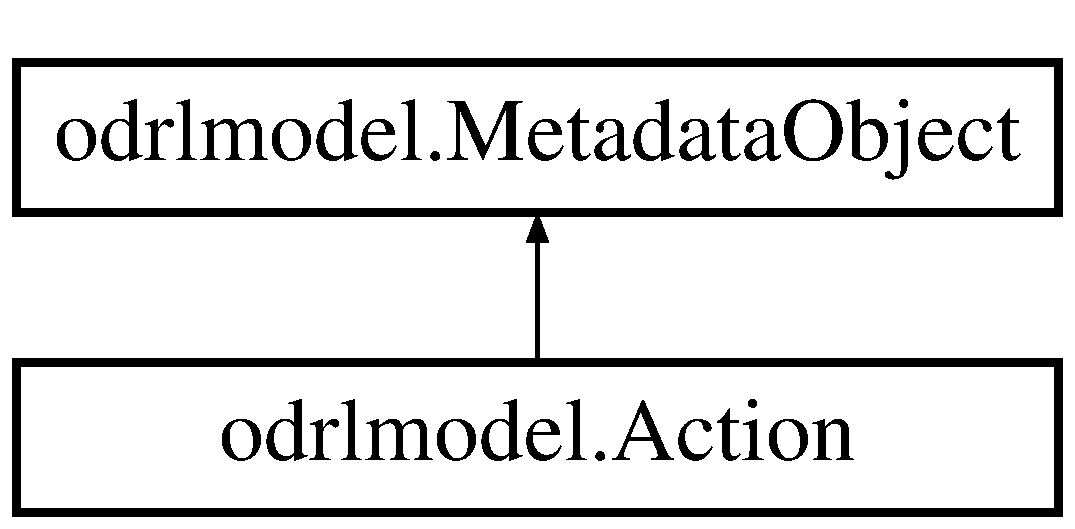
\includegraphics[height=2.000000cm]{classodrlmodel_1_1_action}
\end{center}
\end{figure}
\subsection*{Public Member Functions}
\begin{DoxyCompactItemize}
\item 
\hyperlink{classodrlmodel_1_1_action_aba2aea2da231fcdfa327f82f9408a2ac}{Action} ()
\item 
\hyperlink{classodrlmodel_1_1_action_a8b58d562806a42c51959f257cbc5e8c8}{Action} (\hyperlink{classodrlmodel_1_1_action}{Action} a)
\item 
\hyperlink{classodrlmodel_1_1_action_a94997efd5b4b9b2c6baa428767199e41}{Action} (String \-\_\-uri)
\end{DoxyCompactItemize}
\subsection*{Additional Inherited Members}


\subsection{Detailed Description}
This class represents an O\-D\-R\-L \hyperlink{classodrlmodel_1_1_action}{Action}.

The \hyperlink{classodrlmodel_1_1_action}{Action} entity (when related to a \hyperlink{classodrlmodel_1_1_permission}{Permission} entity) indicates the operations (e.\-g. play, copy, etc.) that the assignee (i.\-e. the consumer) is permitted to perform on the related \hyperlink{classodrlmodel_1_1_asset}{Asset} linked to by \hyperlink{classodrlmodel_1_1_permission}{Permission}.

When related to a \hyperlink{classodrlmodel_1_1_prohibition}{Prohibition}, the \hyperlink{classodrlmodel_1_1_action}{Action} entity indicates the operations that the assignee (again the consumer) is prohibited to perform on the \hyperlink{classodrlmodel_1_1_asset}{Asset} linked to by \hyperlink{classodrlmodel_1_1_prohibition}{Prohibition}. Analogously, when related to a \hyperlink{classodrlmodel_1_1_duty}{Duty}, it indicates the operation to be performed. \hyperlink{classodrlmodel_1_1_action}{Action} contains the following attribute\-: name\-: indicates the \hyperlink{classodrlmodel_1_1_action}{Action} entity term (R\-E\-Q\-U\-I\-R\-E\-D) As its value, the name attribute M\-A\-Y take one of a set of \hyperlink{classodrlmodel_1_1_action}{Action} names which are formally defined in profiles.

The O\-D\-R\-L Common Vocabulary defines a standard set of potential terms that M\-A\-Y be used. For example\-: 
\begin{DoxyItemize}
\item \href{http://www.w3.org/ns/odrl/2/write}{\tt http\-://www.\-w3.\-org/ns/odrl/2/write} 
\item \href{http://www.w3.org/ns/odrl/2/read}{\tt http\-://www.\-w3.\-org/ns/odrl/2/read} 
\item \href{http://www.w3.org/ns/odrl/2/distribute}{\tt http\-://www.\-w3.\-org/ns/odrl/2/distribute} 
\end{DoxyItemize}

Communities will develop new (or extend existing) profiles to capture additional and refined semantics. \begin{DoxyAuthor}{Author}
Victor Rodriguez Doncel at O\-E\-G-\/\-U\-P\-M 2014 
\end{DoxyAuthor}


\subsection{Constructor \& Destructor Documentation}
\hypertarget{classodrlmodel_1_1_action_aba2aea2da231fcdfa327f82f9408a2ac}{\index{odrlmodel\-::\-Action@{odrlmodel\-::\-Action}!Action@{Action}}
\index{Action@{Action}!odrlmodel::Action@{odrlmodel\-::\-Action}}
\subsubsection[{Action}]{\setlength{\rightskip}{0pt plus 5cm}odrlmodel.\-Action.\-Action (
\begin{DoxyParamCaption}
{}
\end{DoxyParamCaption}
)}}\label{classodrlmodel_1_1_action_aba2aea2da231fcdfa327f82f9408a2ac}
\hyperlink{classodrlmodel_1_1_action}{Action} constructor with a random U\-R\-I in the default namespace. By default, an action will be like this\-: \href{http://salonica.dia.fi.upm.es/ldr/action/2e7de960-7001-4c07-bde5-c5ad1f35133d}{\tt http\-://salonica.\-dia.\-fi.\-upm.\-es/ldr/action/2e7de960-\/7001-\/4c07-\/bde5-\/c5ad1f35133d} \hypertarget{classodrlmodel_1_1_action_a8b58d562806a42c51959f257cbc5e8c8}{\index{odrlmodel\-::\-Action@{odrlmodel\-::\-Action}!Action@{Action}}
\index{Action@{Action}!odrlmodel::Action@{odrlmodel\-::\-Action}}
\subsubsection[{Action}]{\setlength{\rightskip}{0pt plus 5cm}odrlmodel.\-Action.\-Action (
\begin{DoxyParamCaption}
\item[{{\bf Action}}]{a}
\end{DoxyParamCaption}
)}}\label{classodrlmodel_1_1_action_a8b58d562806a42c51959f257cbc5e8c8}
Cloner constructor \hypertarget{classodrlmodel_1_1_action_a94997efd5b4b9b2c6baa428767199e41}{\index{odrlmodel\-::\-Action@{odrlmodel\-::\-Action}!Action@{Action}}
\index{Action@{Action}!odrlmodel::Action@{odrlmodel\-::\-Action}}
\subsubsection[{Action}]{\setlength{\rightskip}{0pt plus 5cm}odrlmodel.\-Action.\-Action (
\begin{DoxyParamCaption}
\item[{String}]{\-\_\-uri}
\end{DoxyParamCaption}
)}}\label{classodrlmodel_1_1_action_a94997efd5b4b9b2c6baa428767199e41}
Creates an action identified by the given U\-R\-I. This \hyperlink{classodrlmodel_1_1_action}{Action} might be one of those defined by O\-D\-R\-L, in which case label, comment, and see\-Also are loaded from the O\-D\-R\-L ontology 
\begin{DoxyParams}{Parameters}
{\em \-\_\-uri} & U\-R\-I of the action \\
\hline
\end{DoxyParams}


The documentation for this class was generated from the following file\-:\begin{DoxyCompactItemize}
\item 
src/odrlmodel/Action.\-java\end{DoxyCompactItemize}

\hypertarget{classodrlmodel_1_1_asset}{\section{odrlmodel.\-Asset Class Reference}
\label{classodrlmodel_1_1_asset}\index{odrlmodel.\-Asset@{odrlmodel.\-Asset}}
}
Inheritance diagram for odrlmodel.\-Asset\-:\begin{figure}[H]
\begin{center}
\leavevmode
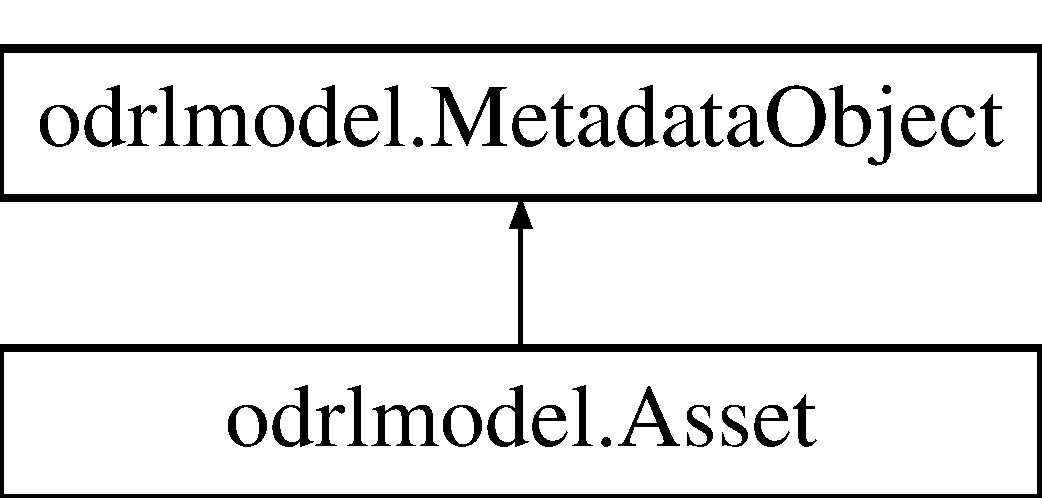
\includegraphics[height=2.000000cm]{classodrlmodel_1_1_asset}
\end{center}
\end{figure}
\subsection*{Public Member Functions}
\begin{DoxyCompactItemize}
\item 
\hyperlink{classodrlmodel_1_1_asset_a6a77e36bcdfc41e612c3fcaf262fb8c1}{Asset} ()
\item 
\hyperlink{classodrlmodel_1_1_asset_a066f7b7be939762221ad48418df105ee}{Asset} (String s)
\item 
List$<$ \hyperlink{classodrlmodel_1_1_policy}{Policy} $>$ \hyperlink{classodrlmodel_1_1_asset_a8e24d6038216a50ab4263cf74f5e06c3}{get\-Policies} ()
\item 
void \hyperlink{classodrlmodel_1_1_asset_a436208a27951040627229707fbdc9020}{set\-Policy} (\hyperlink{classodrlmodel_1_1_policy}{Policy} policy)
\item 
void \hyperlink{classodrlmodel_1_1_asset_a672387d6310a34ab8494ca3a3f9838d5}{add\-Policy} (\hyperlink{classodrlmodel_1_1_policy}{Policy} policy)
\item 
void \hyperlink{classodrlmodel_1_1_asset_abe1e947ddc4d09cbf4058c78ec468b52}{remove\-Policy} (String uri)
\end{DoxyCompactItemize}
\subsection*{Public Attributes}
\begin{DoxyCompactItemize}
\item 
List$<$ \hyperlink{classodrlmodel_1_1_policy}{Policy} $>$ \hyperlink{classodrlmodel_1_1_asset_a140b2ed540257e126a199ee6982a7d69}{policies} = new Array\-List()
\end{DoxyCompactItemize}
\subsection*{Additional Inherited Members}


\subsection{Detailed Description}
This class represents an O\-D\-R\-L 2.\-0 \hyperlink{classodrlmodel_1_1_asset}{Asset}

The \hyperlink{classodrlmodel_1_1_asset}{Asset} entity is aimed at identifying the content that is the subject of an O\-D\-R\-L policy, e.\-g. a media file or ebook. Furthermore, it can be used to represent other \hyperlink{classodrlmodel_1_1_asset}{Asset} entities that are needed to undertake the \hyperlink{classodrlmodel_1_1_policy}{Policy} expression, such as with the \hyperlink{classodrlmodel_1_1_duty}{Duty} entity.

The \hyperlink{classodrlmodel_1_1_asset}{Asset} entity is referred to by the \hyperlink{classodrlmodel_1_1_permission}{Permission} and/or \hyperlink{classodrlmodel_1_1_prohibition}{Prohibition} entities, and also by the \hyperlink{classodrlmodel_1_1_duty}{Duty} entity. The \hyperlink{classodrlmodel_1_1_asset}{Asset} entity contains the following attribute\-: uid\-: the unique identification of the \hyperlink{classodrlmodel_1_1_asset}{Asset} (R\-E\-Q\-U\-I\-R\-E\-D)

The identification of the \hyperlink{classodrlmodel_1_1_asset}{Asset} entity is a key foundation of the O\-D\-R\-L \hyperlink{classodrlmodel_1_1_policy}{Policy} language. However, there are some use cases where the O\-D\-R\-L \hyperlink{classodrlmodel_1_1_policy}{Policy} expression M\-A\-Y be embedded inside the target \hyperlink{classodrlmodel_1_1_asset}{Asset}. In these cases, it M\-A\-Y be more appropriate to provide, or infer, a link to the \hyperlink{classodrlmodel_1_1_asset}{Asset} entity (as the complete \hyperlink{classodrlmodel_1_1_asset}{Asset} uid may not be known at the time) through the local context. Use of such inference and context M\-U\-S\-T be documented in the relevant O\-D\-R\-L community Profile.

Since O\-D\-R\-L \-\_\-policies could deal with any kind of asset, the O\-D\-R\-L Core Model does not provide additional metadata to describe \hyperlink{classodrlmodel_1_1_asset}{Asset} entities of particular media types. It is recommended to use already existing metadata standards, such as Dublin Core Metadata Terms that are appropriate to the \hyperlink{classodrlmodel_1_1_asset}{Asset} type or purpose.

The Relation entity is used to associate the \hyperlink{classodrlmodel_1_1_asset}{Asset} entity with the relevant \hyperlink{classodrlmodel_1_1_permission}{Permission}, \hyperlink{classodrlmodel_1_1_prohibition}{Prohibition}, and \hyperlink{classodrlmodel_1_1_duty}{Duty} entities 

\subsection{Constructor \& Destructor Documentation}
\hypertarget{classodrlmodel_1_1_asset_a6a77e36bcdfc41e612c3fcaf262fb8c1}{\index{odrlmodel\-::\-Asset@{odrlmodel\-::\-Asset}!Asset@{Asset}}
\index{Asset@{Asset}!odrlmodel::Asset@{odrlmodel\-::\-Asset}}
\subsubsection[{Asset}]{\setlength{\rightskip}{0pt plus 5cm}odrlmodel.\-Asset.\-Asset (
\begin{DoxyParamCaption}
{}
\end{DoxyParamCaption}
)}}\label{classodrlmodel_1_1_asset_a6a77e36bcdfc41e612c3fcaf262fb8c1}
Creates a Linked Data resource, identifiable by its U\-R\-I. A random U\-R\-I is given. \hypertarget{classodrlmodel_1_1_asset_a066f7b7be939762221ad48418df105ee}{\index{odrlmodel\-::\-Asset@{odrlmodel\-::\-Asset}!Asset@{Asset}}
\index{Asset@{Asset}!odrlmodel::Asset@{odrlmodel\-::\-Asset}}
\subsubsection[{Asset}]{\setlength{\rightskip}{0pt plus 5cm}odrlmodel.\-Asset.\-Asset (
\begin{DoxyParamCaption}
\item[{String}]{s}
\end{DoxyParamCaption}
)}}\label{classodrlmodel_1_1_asset_a066f7b7be939762221ad48418df105ee}
Creates a Linked Data resource, identifiable by its U\-R\-I. 
\begin{DoxyParams}{Parameters}
{\em s} & U\-R\-I of the asset \\
\hline
\end{DoxyParams}


\subsection{Member Function Documentation}
\hypertarget{classodrlmodel_1_1_asset_a672387d6310a34ab8494ca3a3f9838d5}{\index{odrlmodel\-::\-Asset@{odrlmodel\-::\-Asset}!add\-Policy@{add\-Policy}}
\index{add\-Policy@{add\-Policy}!odrlmodel::Asset@{odrlmodel\-::\-Asset}}
\subsubsection[{add\-Policy}]{\setlength{\rightskip}{0pt plus 5cm}void odrlmodel.\-Asset.\-add\-Policy (
\begin{DoxyParamCaption}
\item[{{\bf Policy}}]{policy}
\end{DoxyParamCaption}
)}}\label{classodrlmodel_1_1_asset_a672387d6310a34ab8494ca3a3f9838d5}
Adds a policy to the list of policy 
\begin{DoxyParams}{Parameters}
{\em policy} & New policy to be added \\
\hline
\end{DoxyParams}
\hypertarget{classodrlmodel_1_1_asset_a8e24d6038216a50ab4263cf74f5e06c3}{\index{odrlmodel\-::\-Asset@{odrlmodel\-::\-Asset}!get\-Policies@{get\-Policies}}
\index{get\-Policies@{get\-Policies}!odrlmodel::Asset@{odrlmodel\-::\-Asset}}
\subsubsection[{get\-Policies}]{\setlength{\rightskip}{0pt plus 5cm}List$<${\bf Policy}$>$ odrlmodel.\-Asset.\-get\-Policies (
\begin{DoxyParamCaption}
{}
\end{DoxyParamCaption}
)}}\label{classodrlmodel_1_1_asset_a8e24d6038216a50ab4263cf74f5e06c3}
Returns the list of \-\_\-policies ya completada \begin{DoxyReturn}{Returns}
List of \-\_\-policies 
\end{DoxyReturn}
V\-V\-X\-X\-X\-V\-V\-V \hypertarget{classodrlmodel_1_1_asset_abe1e947ddc4d09cbf4058c78ec468b52}{\index{odrlmodel\-::\-Asset@{odrlmodel\-::\-Asset}!remove\-Policy@{remove\-Policy}}
\index{remove\-Policy@{remove\-Policy}!odrlmodel::Asset@{odrlmodel\-::\-Asset}}
\subsubsection[{remove\-Policy}]{\setlength{\rightskip}{0pt plus 5cm}void odrlmodel.\-Asset.\-remove\-Policy (
\begin{DoxyParamCaption}
\item[{String}]{uri}
\end{DoxyParamCaption}
)}}\label{classodrlmodel_1_1_asset_abe1e947ddc4d09cbf4058c78ec468b52}
Removes the policy of the given U\-R\-I  uri of the policy to be removed \hypertarget{classodrlmodel_1_1_asset_a436208a27951040627229707fbdc9020}{\index{odrlmodel\-::\-Asset@{odrlmodel\-::\-Asset}!set\-Policy@{set\-Policy}}
\index{set\-Policy@{set\-Policy}!odrlmodel::Asset@{odrlmodel\-::\-Asset}}
\subsubsection[{set\-Policy}]{\setlength{\rightskip}{0pt plus 5cm}void odrlmodel.\-Asset.\-set\-Policy (
\begin{DoxyParamCaption}
\item[{{\bf Policy}}]{policy}
\end{DoxyParamCaption}
)}}\label{classodrlmodel_1_1_asset_a436208a27951040627229707fbdc9020}
Sets the given policy as the only policy 
\begin{DoxyParams}{Parameters}
{\em policy} & The policy \\
\hline
\end{DoxyParams}


\subsection{Member Data Documentation}
\hypertarget{classodrlmodel_1_1_asset_a140b2ed540257e126a199ee6982a7d69}{\index{odrlmodel\-::\-Asset@{odrlmodel\-::\-Asset}!policies@{policies}}
\index{policies@{policies}!odrlmodel::Asset@{odrlmodel\-::\-Asset}}
\subsubsection[{policies}]{\setlength{\rightskip}{0pt plus 5cm}List$<${\bf Policy}$>$ odrlmodel.\-Asset.\-policies = new Array\-List()}}\label{classodrlmodel_1_1_asset_a140b2ed540257e126a199ee6982a7d69}
An asseet may have attached a set of \-\_\-policies 

The documentation for this class was generated from the following file\-:\begin{DoxyCompactItemize}
\item 
src/odrlmodel/Asset.\-java\end{DoxyCompactItemize}

\hypertarget{classodrlmodel_1_1_constraint}{\section{odrlmodel.\-Constraint Class Reference}
\label{classodrlmodel_1_1_constraint}\index{odrlmodel.\-Constraint@{odrlmodel.\-Constraint}}
}
Inheritance diagram for odrlmodel.\-Constraint\-:\begin{figure}[H]
\begin{center}
\leavevmode
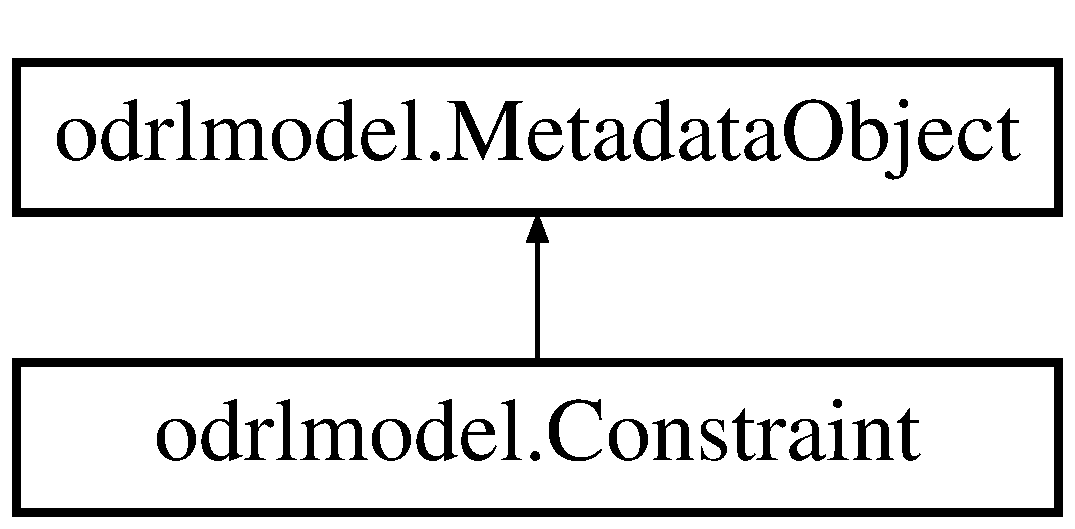
\includegraphics[height=2.000000cm]{classodrlmodel_1_1_constraint}
\end{center}
\end{figure}
\subsection*{Public Member Functions}
\begin{DoxyCompactItemize}
\item 
\hyperlink{classodrlmodel_1_1_constraint_adb03e20fbc5184936dc849508e8a9e02}{Constraint} ()
\item 
\hyperlink{classodrlmodel_1_1_constraint_a540f08813d46fd9e006d1f19fa1e5139}{Constraint} (\hyperlink{classodrlmodel_1_1_constraint}{Constraint} copia)
\item 
\hyperlink{classodrlmodel_1_1_constraint_a3a4d2d03c916c0b5c51de568a43d9761}{Constraint} (String \-\_\-uri)
\item 
void \hyperlink{classodrlmodel_1_1_constraint_a6813d28f7e2eb0375a9247c0c60437ad}{set\-Operator} (String \-\_\-operator)
\item 
void \hyperlink{classodrlmodel_1_1_constraint_a2d0a36345a3a99f683976c5c900f2276}{set\-Right\-Operand} (String \-\_\-right\-Operand)
\item 
void \hyperlink{classodrlmodel_1_1_constraint_a00c68186d9d61ca7c995e260bc595c7b}{set\-Value} (String \-\_\-value)
\end{DoxyCompactItemize}
\subsection*{Protected Attributes}
\begin{DoxyCompactItemize}
\item 
\hypertarget{classodrlmodel_1_1_constraint_af9fac4c8c0805d7eb1f6460f575067fc}{String {\bfseries operator=\char`\"{}\char`\"{}}}\label{classodrlmodel_1_1_constraint_af9fac4c8c0805d7eb1f6460f575067fc}

\item 
\hypertarget{classodrlmodel_1_1_constraint_abde5361d442cd655fb6c5aca3f911fe4}{String {\bfseries right\-Operand} =\char`\"{}\char`\"{}}\label{classodrlmodel_1_1_constraint_abde5361d442cd655fb6c5aca3f911fe4}

\item 
\hypertarget{classodrlmodel_1_1_constraint_a72bbef1fe62aff8d9701c44fa31ef55c}{String {\bfseries value} =\char`\"{}\char`\"{}}\label{classodrlmodel_1_1_constraint_a72bbef1fe62aff8d9701c44fa31ef55c}

\end{DoxyCompactItemize}
\subsection*{Additional Inherited Members}


\subsection{Detailed Description}
This class represents an O\-D\-R\-L2.\-0 \hyperlink{classodrlmodel_1_1_constraint}{Constraint}.

The \hyperlink{classodrlmodel_1_1_constraint}{Constraint} entity indicates limits and restrictions to the \hyperlink{classodrlmodel_1_1_permission}{Permission}, the \hyperlink{classodrlmodel_1_1_prohibition}{Prohibition} and the \hyperlink{classodrlmodel_1_1_duty}{Duty} entity. Constraints express mathematical terms with two operands and one operator. For example, the “number of usages” (name) must be “smaller than” (operator) the “number 10″ (right\-Operand).

If multiple \hyperlink{classodrlmodel_1_1_constraint}{Constraint} entities are linked to the same \hyperlink{classodrlmodel_1_1_permission}{Permission}, \hyperlink{classodrlmodel_1_1_prohibition}{Prohibition}, or \hyperlink{classodrlmodel_1_1_duty}{Duty} entity, then all of the \hyperlink{classodrlmodel_1_1_constraint}{Constraint} entities M\-U\-S\-T be satisfied. That is, all the \hyperlink{classodrlmodel_1_1_constraint}{Constraint} entities are (boolean) anded. In the case where the same \hyperlink{classodrlmodel_1_1_constraint}{Constraint} is repeated, then these M\-U\-S\-T be represented as a single \hyperlink{classodrlmodel_1_1_constraint}{Constraint} entity using an appropriate operator value (for example, is\-Any\-Of).

\begin{DoxyAuthor}{Author}
Victor Rodriguez Doncel at O\-E\-G-\/\-U\-P\-M 2014 
\end{DoxyAuthor}


\subsection{Constructor \& Destructor Documentation}
\hypertarget{classodrlmodel_1_1_constraint_adb03e20fbc5184936dc849508e8a9e02}{\index{odrlmodel\-::\-Constraint@{odrlmodel\-::\-Constraint}!Constraint@{Constraint}}
\index{Constraint@{Constraint}!odrlmodel::Constraint@{odrlmodel\-::\-Constraint}}
\subsubsection[{Constraint}]{\setlength{\rightskip}{0pt plus 5cm}odrlmodel.\-Constraint.\-Constraint (
\begin{DoxyParamCaption}
{}
\end{DoxyParamCaption}
)}}\label{classodrlmodel_1_1_constraint_adb03e20fbc5184936dc849508e8a9e02}
Default constraint with a random U\-R\-I \hypertarget{classodrlmodel_1_1_constraint_a540f08813d46fd9e006d1f19fa1e5139}{\index{odrlmodel\-::\-Constraint@{odrlmodel\-::\-Constraint}!Constraint@{Constraint}}
\index{Constraint@{Constraint}!odrlmodel::Constraint@{odrlmodel\-::\-Constraint}}
\subsubsection[{Constraint}]{\setlength{\rightskip}{0pt plus 5cm}odrlmodel.\-Constraint.\-Constraint (
\begin{DoxyParamCaption}
\item[{{\bf Constraint}}]{copia}
\end{DoxyParamCaption}
)}}\label{classodrlmodel_1_1_constraint_a540f08813d46fd9e006d1f19fa1e5139}
Cloner constructor \hypertarget{classodrlmodel_1_1_constraint_a3a4d2d03c916c0b5c51de568a43d9761}{\index{odrlmodel\-::\-Constraint@{odrlmodel\-::\-Constraint}!Constraint@{Constraint}}
\index{Constraint@{Constraint}!odrlmodel::Constraint@{odrlmodel\-::\-Constraint}}
\subsubsection[{Constraint}]{\setlength{\rightskip}{0pt plus 5cm}odrlmodel.\-Constraint.\-Constraint (
\begin{DoxyParamCaption}
\item[{String}]{\-\_\-uri}
\end{DoxyParamCaption}
)}}\label{classodrlmodel_1_1_constraint_a3a4d2d03c916c0b5c51de568a43d9761}
Creates an action identified by the given U\-R\-I. This \hyperlink{classodrlmodel_1_1_action}{Action} might be one of those defined by O\-D\-R\-L, in which case label, comment, and see\-Also are loaded from the O\-D\-R\-L ontology 
\begin{DoxyParams}{Parameters}
{\em \-\_\-uri} & U\-R\-I of the action \\
\hline
\end{DoxyParams}


\subsection{Member Function Documentation}
\hypertarget{classodrlmodel_1_1_constraint_a6813d28f7e2eb0375a9247c0c60437ad}{\index{odrlmodel\-::\-Constraint@{odrlmodel\-::\-Constraint}!set\-Operator@{set\-Operator}}
\index{set\-Operator@{set\-Operator}!odrlmodel::Constraint@{odrlmodel\-::\-Constraint}}
\subsubsection[{set\-Operator}]{\setlength{\rightskip}{0pt plus 5cm}void odrlmodel.\-Constraint.\-set\-Operator (
\begin{DoxyParamCaption}
\item[{String}]{\-\_\-operator}
\end{DoxyParamCaption}
)}}\label{classodrlmodel_1_1_constraint_a6813d28f7e2eb0375a9247c0c60437ad}
Sets the operator 
\begin{DoxyParams}{Parameters}
{\em \-\_\-operator} & An operator, like \href{http://www.w3.org/ns/odrl/2/gt}{\tt http\-://www.\-w3.\-org/ns/odrl/2/gt} or \href{http://www.w3.org/ns/odrl/2/eq}{\tt http\-://www.\-w3.\-org/ns/odrl/2/eq} \\
\hline
\end{DoxyParams}
\hypertarget{classodrlmodel_1_1_constraint_a2d0a36345a3a99f683976c5c900f2276}{\index{odrlmodel\-::\-Constraint@{odrlmodel\-::\-Constraint}!set\-Right\-Operand@{set\-Right\-Operand}}
\index{set\-Right\-Operand@{set\-Right\-Operand}!odrlmodel::Constraint@{odrlmodel\-::\-Constraint}}
\subsubsection[{set\-Right\-Operand}]{\setlength{\rightskip}{0pt plus 5cm}void odrlmodel.\-Constraint.\-set\-Right\-Operand (
\begin{DoxyParamCaption}
\item[{String}]{\-\_\-right\-Operand}
\end{DoxyParamCaption}
)}}\label{classodrlmodel_1_1_constraint_a2d0a36345a3a99f683976c5c900f2276}
Sets the right\-Operand 
\begin{DoxyParams}{Parameters}
{\em \-\_\-right\-Operand} & A right\-Operand, like \href{http://www.w3.org/ns/odrl/2/language,}{\tt http\-://www.\-w3.\-org/ns/odrl/2/language,} \href{http://www.w3.org/ns/odrl/2/industry,}{\tt http\-://www.\-w3.\-org/ns/odrl/2/industry,} etc. \\
\hline
\end{DoxyParams}
\hypertarget{classodrlmodel_1_1_constraint_a00c68186d9d61ca7c995e260bc595c7b}{\index{odrlmodel\-::\-Constraint@{odrlmodel\-::\-Constraint}!set\-Value@{set\-Value}}
\index{set\-Value@{set\-Value}!odrlmodel::Constraint@{odrlmodel\-::\-Constraint}}
\subsubsection[{set\-Value}]{\setlength{\rightskip}{0pt plus 5cm}void odrlmodel.\-Constraint.\-set\-Value (
\begin{DoxyParamCaption}
\item[{String}]{\-\_\-value}
\end{DoxyParamCaption}
)}}\label{classodrlmodel_1_1_constraint_a00c68186d9d61ca7c995e260bc595c7b}
Sets the vlue 
\begin{DoxyParams}{Parameters}
{\em \-\_\-value} & Value, like \href{http://www.lexvo.org/page/iso639-3/eng,}{\tt http\-://www.\-lexvo.\-org/page/iso639-\/3/eng,} 3, etc. \\
\hline
\end{DoxyParams}


The documentation for this class was generated from the following file\-:\begin{DoxyCompactItemize}
\item 
src/odrlmodel/Constraint.\-java\end{DoxyCompactItemize}

\hypertarget{classodrlmodel_1_1_duty}{\section{odrlmodel.\-Duty Class Reference}
\label{classodrlmodel_1_1_duty}\index{odrlmodel.\-Duty@{odrlmodel.\-Duty}}
}
Inheritance diagram for odrlmodel.\-Duty\-:\begin{figure}[H]
\begin{center}
\leavevmode
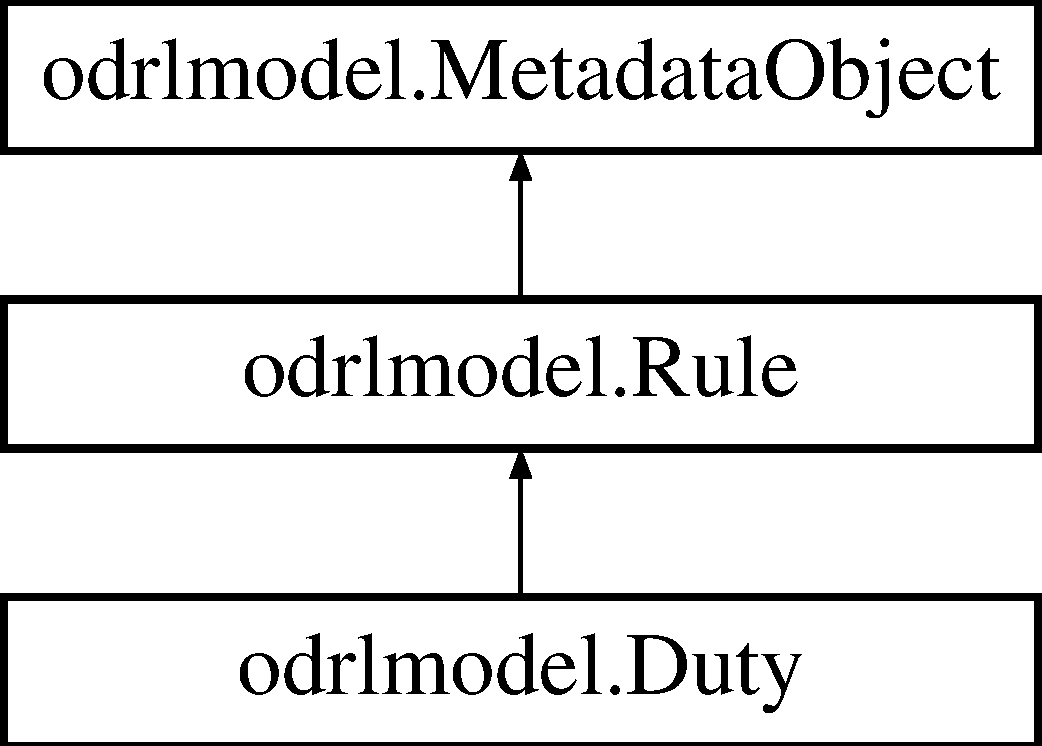
\includegraphics[height=3.000000cm]{classodrlmodel_1_1_duty}
\end{center}
\end{figure}
\subsection*{Public Member Functions}
\begin{DoxyCompactItemize}
\item 
\hyperlink{classodrlmodel_1_1_duty_a9451204912dfac8559df1489573a7776}{Duty} (String \-\_\-uri)
\end{DoxyCompactItemize}
\subsection*{Additional Inherited Members}


\subsection{Detailed Description}
This class represents an O\-D\-R\-L2.\-0 \hyperlink{classodrlmodel_1_1_duty}{Duty} The \hyperlink{classodrlmodel_1_1_duty}{Duty} entity indicates a requirement that M\-A\-Y be fulfilled in return for being entitled to the referring \hyperlink{classodrlmodel_1_1_permission}{Permission} entity.

While implying different semantics, the \hyperlink{classodrlmodel_1_1_duty}{Duty} entity is similar to \hyperlink{classodrlmodel_1_1_permission}{Permission} in that it is an \hyperlink{classodrlmodel_1_1_action}{Action} that can be undertaken. If a \hyperlink{classodrlmodel_1_1_permission}{Permission} refers to several \hyperlink{classodrlmodel_1_1_duty}{Duty} entities, all of them have to be fulfilled for the \hyperlink{classodrlmodel_1_1_permission}{Permission} to become valid. If several \hyperlink{classodrlmodel_1_1_permission}{Permission} entities refer to one \hyperlink{classodrlmodel_1_1_duty}{Duty}, then the \hyperlink{classodrlmodel_1_1_duty}{Duty} only has to be fulfilled once for all the \hyperlink{classodrlmodel_1_1_permission}{Permission} entities to become valid.

\begin{DoxyAuthor}{Author}
Victor Rodriguez Doncel at O\-E\-G-\/\-U\-P\-M 2014 
\end{DoxyAuthor}


\subsection{Constructor \& Destructor Documentation}
\hypertarget{classodrlmodel_1_1_duty_a9451204912dfac8559df1489573a7776}{\index{odrlmodel\-::\-Duty@{odrlmodel\-::\-Duty}!Duty@{Duty}}
\index{Duty@{Duty}!odrlmodel::Duty@{odrlmodel\-::\-Duty}}
\subsubsection[{Duty}]{\setlength{\rightskip}{0pt plus 5cm}odrlmodel.\-Duty.\-Duty (
\begin{DoxyParamCaption}
\item[{String}]{\-\_\-uri}
\end{DoxyParamCaption}
)}}\label{classodrlmodel_1_1_duty_a9451204912dfac8559df1489573a7776}
Creates a duty identified by the given U\-R\-I. 
\begin{DoxyParams}{Parameters}
{\em \-\_\-uri} & U\-R\-I of the duty \\
\hline
\end{DoxyParams}


The documentation for this class was generated from the following file\-:\begin{DoxyCompactItemize}
\item 
src/odrlmodel/Duty.\-java\end{DoxyCompactItemize}

\hypertarget{classodrlmodel_1_1_l_d_r_config}{\section{odrlmodel.\-L\-D\-R\-Config Class Reference}
\label{classodrlmodel_1_1_l_d_r_config}\index{odrlmodel.\-L\-D\-R\-Config@{odrlmodel.\-L\-D\-R\-Config}}
}
\subsection*{Public Member Functions}
\begin{DoxyCompactItemize}
\item 
\hypertarget{classodrlmodel_1_1_l_d_r_config_a0b0b9c8d753bad13072439d9ab6b4c19}{void {\bfseries set\-Dataset} (String str)}\label{classodrlmodel_1_1_l_d_r_config_a0b0b9c8d753bad13072439d9ab6b4c19}

\end{DoxyCompactItemize}
\subsection*{Static Public Member Functions}
\begin{DoxyCompactItemize}
\item 
static void \hyperlink{classodrlmodel_1_1_l_d_r_config_a03eaf649f790ca3b179cbcffe94cbba6}{insert\-Param\-Value} (String nomparam, int id\-Elem\-Cons, int valor)
\item 
static int \hyperlink{classodrlmodel_1_1_l_d_r_config_a7f1ac9e32800dade8fc82a175b0717f1}{get\-Param\-Value} (String nomparam, int id\-Elem\-Cons)
\item 
static String \hyperlink{classodrlmodel_1_1_l_d_r_config_a5fc3ec8c96ab3388a637452d6badcfaf}{get} (String p)
\item 
static String \hyperlink{classodrlmodel_1_1_l_d_r_config_a08787eb61b126f83df29739b625cfdb5}{get} (String p, String valor)
\item 
static void \hyperlink{classodrlmodel_1_1_l_d_r_config_ada42c1a12fce0abe6e88371f00bdefc3}{set} (String p, String defvalue)
\item 
\hypertarget{classodrlmodel_1_1_l_d_r_config_aea1018bbe406316722f5915c4951c536}{static String {\bfseries get\-Authorizebydefault} ()}\label{classodrlmodel_1_1_l_d_r_config_aea1018bbe406316722f5915c4951c536}

\item 
\hypertarget{classodrlmodel_1_1_l_d_r_config_acd3a1eaf2162552ecbe7afd5b7daadb0}{static void {\bfseries set\-Authorizebydefault} (String num\-Bins)}\label{classodrlmodel_1_1_l_d_r_config_acd3a1eaf2162552ecbe7afd5b7daadb0}

\item 
\hypertarget{classodrlmodel_1_1_l_d_r_config_ab83adab4709644be8ddc4751cdb51d05}{static String {\bfseries get\-Keystore} ()}\label{classodrlmodel_1_1_l_d_r_config_ab83adab4709644be8ddc4751cdb51d05}

\item 
\hypertarget{classodrlmodel_1_1_l_d_r_config_adbf32274b89387ebd0d4a2d65252fd93}{static void {\bfseries set\-Keystore} (String num\-Bins)}\label{classodrlmodel_1_1_l_d_r_config_adbf32274b89387ebd0d4a2d65252fd93}

\item 
\hypertarget{classodrlmodel_1_1_l_d_r_config_a934733508d61f5b7ae0b12eb0504a60c}{static String {\bfseries get\-Licensesfolder} ()}\label{classodrlmodel_1_1_l_d_r_config_a934733508d61f5b7ae0b12eb0504a60c}

\item 
\hypertarget{classodrlmodel_1_1_l_d_r_config_ac248ad38107a413d189ec7ad5ab33080}{static void {\bfseries set\-Licensesfolder} (String str)}\label{classodrlmodel_1_1_l_d_r_config_ac248ad38107a413d189ec7ad5ab33080}

\item 
\hypertarget{classodrlmodel_1_1_l_d_r_config_aa85688ec7f9d2c5f66d9eccb4e3a666c}{static String {\bfseries get\-Datafolder} ()}\label{classodrlmodel_1_1_l_d_r_config_aa85688ec7f9d2c5f66d9eccb4e3a666c}

\item 
\hypertarget{classodrlmodel_1_1_l_d_r_config_a795aa6f80d07d61d065a702fba948c58}{static void {\bfseries set\-Datafolder} (String num\-Bins)}\label{classodrlmodel_1_1_l_d_r_config_a795aa6f80d07d61d065a702fba948c58}

\item 
\hypertarget{classodrlmodel_1_1_l_d_r_config_aca15535c8d52e1c39fdbb73235da992e}{static String {\bfseries get\-Policyassetstore} ()}\label{classodrlmodel_1_1_l_d_r_config_aca15535c8d52e1c39fdbb73235da992e}

\item 
\hypertarget{classodrlmodel_1_1_l_d_r_config_a503e0e3584e7703673613ea417c71367}{static void {\bfseries set\-Policyassetstore} (String num\-Bins)}\label{classodrlmodel_1_1_l_d_r_config_a503e0e3584e7703673613ea417c71367}

\item 
\hypertarget{classodrlmodel_1_1_l_d_r_config_a6049dff069291802408fed46e07fc184}{static void {\bfseries set\-Namespace} (String str)}\label{classodrlmodel_1_1_l_d_r_config_a6049dff069291802408fed46e07fc184}

\item 
\hypertarget{classodrlmodel_1_1_l_d_r_config_ac3cb7acc863a348f5e3de1dd799ac2d3}{static String {\bfseries get\-Namespace} ()}\label{classodrlmodel_1_1_l_d_r_config_ac3cb7acc863a348f5e3de1dd799ac2d3}

\item 
\hypertarget{classodrlmodel_1_1_l_d_r_config_a103e323035ac8aa9b8d70ce9646e40ee}{static void {\bfseries set\-Server} (String str)}\label{classodrlmodel_1_1_l_d_r_config_a103e323035ac8aa9b8d70ce9646e40ee}

\item 
\hypertarget{classodrlmodel_1_1_l_d_r_config_a10f77cd552226d582c1ec4b9bec8a591}{static String {\bfseries get\-Server} ()}\label{classodrlmodel_1_1_l_d_r_config_a10f77cd552226d582c1ec4b9bec8a591}

\item 
\hypertarget{classodrlmodel_1_1_l_d_r_config_a9b86027da393b55c7f6bf988c99a90e5}{static void {\bfseries set\-Port} (String str)}\label{classodrlmodel_1_1_l_d_r_config_a9b86027da393b55c7f6bf988c99a90e5}

\item 
\hypertarget{classodrlmodel_1_1_l_d_r_config_accd00c860dea0b5b15663fa205761e12}{static String {\bfseries get\-Port} ()}\label{classodrlmodel_1_1_l_d_r_config_accd00c860dea0b5b15663fa205761e12}

\item 
\hypertarget{classodrlmodel_1_1_l_d_r_config_a62ecf5e5299d46f77bacf5c31473b3db}{static String {\bfseries get\-Dataset} ()}\label{classodrlmodel_1_1_l_d_r_config_a62ecf5e5299d46f77bacf5c31473b3db}

\item 
static boolean \hyperlink{classodrlmodel_1_1_l_d_r_config_aa98419a5b5f87f457bb176035986d439}{Load} ()
\item 
static void \hyperlink{classodrlmodel_1_1_l_d_r_config_a9a89297e7d7ce894a22a3087f11c9af4}{Store} ()
\end{DoxyCompactItemize}


\subsection{Detailed Description}
Reads and writes parameters in a configfile

El archivo es {\itshape \char`\"{}ldr.\-config\char`\"{}} y debe estar en la misma carpeta que el jar Parámetros (ejemplo)\-: \begin{DoxyAuthor}{Author}
Victor Rodriguez Doncel 
\end{DoxyAuthor}


\subsection{Member Function Documentation}
\hypertarget{classodrlmodel_1_1_l_d_r_config_a5fc3ec8c96ab3388a637452d6badcfaf}{\index{odrlmodel\-::\-L\-D\-R\-Config@{odrlmodel\-::\-L\-D\-R\-Config}!get@{get}}
\index{get@{get}!odrlmodel::LDRConfig@{odrlmodel\-::\-L\-D\-R\-Config}}
\subsubsection[{get}]{\setlength{\rightskip}{0pt plus 5cm}static String odrlmodel.\-L\-D\-R\-Config.\-get (
\begin{DoxyParamCaption}
\item[{String}]{p}
\end{DoxyParamCaption}
)\hspace{0.3cm}{\ttfamily [static]}}}\label{classodrlmodel_1_1_l_d_r_config_a5fc3ec8c96ab3388a637452d6badcfaf}
Obtiene el valor de una propiedad 
\begin{DoxyParams}{Parameters}
{\em p} & Propiedad \\
\hline
\end{DoxyParams}
\hypertarget{classodrlmodel_1_1_l_d_r_config_a08787eb61b126f83df29739b625cfdb5}{\index{odrlmodel\-::\-L\-D\-R\-Config@{odrlmodel\-::\-L\-D\-R\-Config}!get@{get}}
\index{get@{get}!odrlmodel::LDRConfig@{odrlmodel\-::\-L\-D\-R\-Config}}
\subsubsection[{get}]{\setlength{\rightskip}{0pt plus 5cm}static String odrlmodel.\-L\-D\-R\-Config.\-get (
\begin{DoxyParamCaption}
\item[{String}]{p, }
\item[{String}]{valor}
\end{DoxyParamCaption}
)\hspace{0.3cm}{\ttfamily [static]}}}\label{classodrlmodel_1_1_l_d_r_config_a08787eb61b126f83df29739b625cfdb5}
Obtiene el valor de una propiedad, y si no lo tiene da un valor por defecto 
\begin{DoxyParams}{Parameters}
{\em p} & Propiedad \\
\hline
{\em valor} & Valor por defecto \\
\hline
\end{DoxyParams}
\begin{DoxyReturn}{Returns}
El valor leido o el de por defecto 
\end{DoxyReturn}
\hypertarget{classodrlmodel_1_1_l_d_r_config_a7f1ac9e32800dade8fc82a175b0717f1}{\index{odrlmodel\-::\-L\-D\-R\-Config@{odrlmodel\-::\-L\-D\-R\-Config}!get\-Param\-Value@{get\-Param\-Value}}
\index{get\-Param\-Value@{get\-Param\-Value}!odrlmodel::LDRConfig@{odrlmodel\-::\-L\-D\-R\-Config}}
\subsubsection[{get\-Param\-Value}]{\setlength{\rightskip}{0pt plus 5cm}static int odrlmodel.\-L\-D\-R\-Config.\-get\-Param\-Value (
\begin{DoxyParamCaption}
\item[{String}]{nomparam, }
\item[{int}]{id\-Elem\-Cons}
\end{DoxyParamCaption}
)\hspace{0.3cm}{\ttfamily [static]}}}\label{classodrlmodel_1_1_l_d_r_config_a7f1ac9e32800dade8fc82a175b0717f1}
Obtiene el valor de un parámetro para un elemento consumidor. 
\begin{DoxyParams}{Parameters}
{\em nomparam} & Nombre del parámetro \\
\hline
{\em id\-Elem\-Cons} & Identificador del elemento consumidor \\
\hline
\end{DoxyParams}
\begin{DoxyReturn}{Returns}
Un valor numérico 
\end{DoxyReturn}
\hypertarget{classodrlmodel_1_1_l_d_r_config_a03eaf649f790ca3b179cbcffe94cbba6}{\index{odrlmodel\-::\-L\-D\-R\-Config@{odrlmodel\-::\-L\-D\-R\-Config}!insert\-Param\-Value@{insert\-Param\-Value}}
\index{insert\-Param\-Value@{insert\-Param\-Value}!odrlmodel::LDRConfig@{odrlmodel\-::\-L\-D\-R\-Config}}
\subsubsection[{insert\-Param\-Value}]{\setlength{\rightskip}{0pt plus 5cm}static void odrlmodel.\-L\-D\-R\-Config.\-insert\-Param\-Value (
\begin{DoxyParamCaption}
\item[{String}]{nomparam, }
\item[{int}]{id\-Elem\-Cons, }
\item[{int}]{valor}
\end{DoxyParamCaption}
)\hspace{0.3cm}{\ttfamily [static]}}}\label{classodrlmodel_1_1_l_d_r_config_a03eaf649f790ca3b179cbcffe94cbba6}
Inserta el valor de un parámetro para un elemento consumidor. 
\begin{DoxyParams}{Parameters}
{\em nomparam} & Nombre del parámetro \\
\hline
{\em id\-Elem\-Cons} & Id del elemento consumidor \\
\hline
{\em valor} & Valor \\
\hline
\end{DoxyParams}
\hypertarget{classodrlmodel_1_1_l_d_r_config_aa98419a5b5f87f457bb176035986d439}{\index{odrlmodel\-::\-L\-D\-R\-Config@{odrlmodel\-::\-L\-D\-R\-Config}!Load@{Load}}
\index{Load@{Load}!odrlmodel::LDRConfig@{odrlmodel\-::\-L\-D\-R\-Config}}
\subsubsection[{Load}]{\setlength{\rightskip}{0pt plus 5cm}static boolean odrlmodel.\-L\-D\-R\-Config.\-Load (
\begin{DoxyParamCaption}
{}
\end{DoxyParamCaption}
)\hspace{0.3cm}{\ttfamily [static]}}}\label{classodrlmodel_1_1_l_d_r_config_aa98419a5b5f87f457bb176035986d439}
Carga los parametros de configuracion del archivo contenidos.\-config \begin{DoxyReturn}{Returns}
True si todo fue bien 
\end{DoxyReturn}
\hypertarget{classodrlmodel_1_1_l_d_r_config_ada42c1a12fce0abe6e88371f00bdefc3}{\index{odrlmodel\-::\-L\-D\-R\-Config@{odrlmodel\-::\-L\-D\-R\-Config}!set@{set}}
\index{set@{set}!odrlmodel::LDRConfig@{odrlmodel\-::\-L\-D\-R\-Config}}
\subsubsection[{set}]{\setlength{\rightskip}{0pt plus 5cm}static void odrlmodel.\-L\-D\-R\-Config.\-set (
\begin{DoxyParamCaption}
\item[{String}]{p, }
\item[{String}]{defvalue}
\end{DoxyParamCaption}
)\hspace{0.3cm}{\ttfamily [static]}}}\label{classodrlmodel_1_1_l_d_r_config_ada42c1a12fce0abe6e88371f00bdefc3}
Estable el valor de una propiedad 
\begin{DoxyParams}{Parameters}
{\em p} & Propiedad \\
\hline
{\em valor} & Valor \\
\hline
\end{DoxyParams}
\hypertarget{classodrlmodel_1_1_l_d_r_config_a9a89297e7d7ce894a22a3087f11c9af4}{\index{odrlmodel\-::\-L\-D\-R\-Config@{odrlmodel\-::\-L\-D\-R\-Config}!Store@{Store}}
\index{Store@{Store}!odrlmodel::LDRConfig@{odrlmodel\-::\-L\-D\-R\-Config}}
\subsubsection[{Store}]{\setlength{\rightskip}{0pt plus 5cm}static void odrlmodel.\-L\-D\-R\-Config.\-Store (
\begin{DoxyParamCaption}
{}
\end{DoxyParamCaption}
)\hspace{0.3cm}{\ttfamily [static]}}}\label{classodrlmodel_1_1_l_d_r_config_a9a89297e7d7ce894a22a3087f11c9af4}
Almacena los parámetros de configuración en el archivo Este archivo no es configurable El orden de almacenamiento en archivo es alfabético 

The documentation for this class was generated from the following file\-:\begin{DoxyCompactItemize}
\item 
src/odrlmodel/L\-D\-R\-Config.\-java\end{DoxyCompactItemize}

\hypertarget{classodrlmodel_1_1_metadata_object}{\section{odrlmodel.\-Metadata\-Object Class Reference}
\label{classodrlmodel_1_1_metadata_object}\index{odrlmodel.\-Metadata\-Object@{odrlmodel.\-Metadata\-Object}}
}
Inheritance diagram for odrlmodel.\-Metadata\-Object\-:\begin{figure}[H]
\begin{center}
\leavevmode
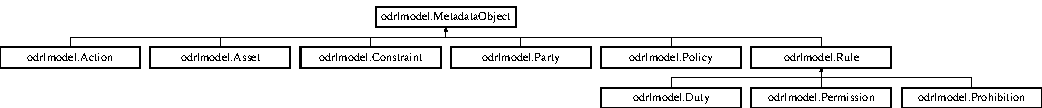
\includegraphics[height=1.428571cm]{classodrlmodel_1_1_metadata_object}
\end{center}
\end{figure}
\subsection*{Public Member Functions}
\begin{DoxyCompactItemize}
\item 
\hyperlink{classodrlmodel_1_1_metadata_object_ab20ea9ece315fa929f47f313c059bb42}{Metadata\-Object} ()
\item 
\hyperlink{classodrlmodel_1_1_metadata_object_a59826bb9a0a9b909b678df4b77008da6}{Metadata\-Object} (String \-\_\-uri)
\item 
\hypertarget{classodrlmodel_1_1_metadata_object_afbc4bcbdf43b341dfcf86e4da445a761}{{\bfseries Metadata\-Object} (\hyperlink{classodrlmodel_1_1_metadata_object}{Metadata\-Object} mo)}\label{classodrlmodel_1_1_metadata_object_afbc4bcbdf43b341dfcf86e4da445a761}

\item 
void \hyperlink{classodrlmodel_1_1_metadata_object_a96bef82bcc0de38aa165c00a6d9d88ec}{set\-U\-R\-I} (String \-\_\-uri)
\item 
String \hyperlink{classodrlmodel_1_1_metadata_object_afe61238df68030c918bf377b91f1f605}{get\-U\-R\-I} ()
\item 
boolean \hyperlink{classodrlmodel_1_1_metadata_object_ae676c6e5f0186acf18bc1426911e16d7}{is\-Anon} ()
\item 
String \hyperlink{classodrlmodel_1_1_metadata_object_a943dfa2720e7c0e773342b6cbec7260f}{get\-Comment} ()
\item 
void \hyperlink{classodrlmodel_1_1_metadata_object_a02b92f7cd561bdbcbf09105a05c6ccbc}{set\-Comment} (String \-\_\-comment)
\item 
String \hyperlink{classodrlmodel_1_1_metadata_object_aef4d6c99e851dc83ccbd1c0672f20ece}{get\-See\-Also} ()
\item 
String \hyperlink{classodrlmodel_1_1_metadata_object_a860de3957bd474683a35f941f1fdc954}{get\-Title} ()
\item 
void \hyperlink{classodrlmodel_1_1_metadata_object_a039dbb6c7887bb53552499bafd42ec54}{set\-Title} (String \-\_\-title)
\item 
String \hyperlink{classodrlmodel_1_1_metadata_object_a9c46072af25fbfc67d14b6329df400ab}{get\-Label} (String lan)
\item 
\hypertarget{classodrlmodel_1_1_metadata_object_ae0abd5d1d2b132dc12bc887f18d8f10e}{void {\bfseries add\-Label} (String label)}\label{classodrlmodel_1_1_metadata_object_ae0abd5d1d2b132dc12bc887f18d8f10e}

\item 
\hypertarget{classodrlmodel_1_1_metadata_object_ad5071d997969db8259edba95f1294f5f}{void {\bfseries set\-Label} (String label, String lang)}\label{classodrlmodel_1_1_metadata_object_ad5071d997969db8259edba95f1294f5f}

\item 
void \hyperlink{classodrlmodel_1_1_metadata_object_a30068a55df0f1053d2e87034f4df574c}{set\-Label} (String \-\_\-label)
\item 
\hypertarget{classodrlmodel_1_1_metadata_object_abaeaaaec78acb676059860c8d22fddfe}{String {\bfseries to\-String} ()}\label{classodrlmodel_1_1_metadata_object_abaeaaaec78acb676059860c8d22fddfe}

\end{DoxyCompactItemize}
\subsection*{Public Attributes}
\begin{DoxyCompactItemize}
\item 
\hypertarget{classodrlmodel_1_1_metadata_object_af0b003dcdfab5da58d765cb0f29a5e77}{List$<$ String $>$ {\bfseries labels} = new Array\-List()}\label{classodrlmodel_1_1_metadata_object_af0b003dcdfab5da58d765cb0f29a5e77}

\item 
\hypertarget{classodrlmodel_1_1_metadata_object_a02b33ee9f1d16129a719bb4d03d0cad6}{String {\bfseries comment} = \char`\"{}\char`\"{}}\label{classodrlmodel_1_1_metadata_object_a02b33ee9f1d16129a719bb4d03d0cad6}

\item 
\hypertarget{classodrlmodel_1_1_metadata_object_a81139568d5481c6045d70714ca4579de}{String {\bfseries see\-Also} =\char`\"{}\char`\"{}}\label{classodrlmodel_1_1_metadata_object_a81139568d5481c6045d70714ca4579de}

\item 
\hypertarget{classodrlmodel_1_1_metadata_object_a3a02e335a5d022de19642dee1c5cd36c}{String {\bfseries title} =\char`\"{}\char`\"{}}\label{classodrlmodel_1_1_metadata_object_a3a02e335a5d022de19642dee1c5cd36c}

\item 
\hypertarget{classodrlmodel_1_1_metadata_object_ab58ebe845c20e917b41b840d4a773683}{String {\bfseries uri} = \char`\"{}\char`\"{}}\label{classodrlmodel_1_1_metadata_object_ab58ebe845c20e917b41b840d4a773683}

\end{DoxyCompactItemize}
\subsection*{Static Public Attributes}
\begin{DoxyCompactItemize}
\item 
\hypertarget{classodrlmodel_1_1_metadata_object_a0b03d4d29c9c15c92e39b371c3cfa841}{static final String {\bfseries D\-E\-F\-A\-U\-L\-T\-\_\-\-N\-A\-M\-E\-S\-P\-A\-C\-E} = L\-D\-R\-Config.\-get\-Namespace()}\label{classodrlmodel_1_1_metadata_object_a0b03d4d29c9c15c92e39b371c3cfa841}

\end{DoxyCompactItemize}


\subsection{Detailed Description}
This class represents a resource with some metadata. Under this simple model, objects may have zero or one metadata elements\-: comments, title, labels or see\-Also Every resource may have a U\-R\-I too, whose default namespace has been made public to be changed at will \begin{DoxyAuthor}{Author}
Victor Rodriguez Doncel at O\-E\-G-\/\-U\-P\-M 2014 
\end{DoxyAuthor}


\subsection{Constructor \& Destructor Documentation}
\hypertarget{classodrlmodel_1_1_metadata_object_ab20ea9ece315fa929f47f313c059bb42}{\index{odrlmodel\-::\-Metadata\-Object@{odrlmodel\-::\-Metadata\-Object}!Metadata\-Object@{Metadata\-Object}}
\index{Metadata\-Object@{Metadata\-Object}!odrlmodel::MetadataObject@{odrlmodel\-::\-Metadata\-Object}}
\subsubsection[{Metadata\-Object}]{\setlength{\rightskip}{0pt plus 5cm}odrlmodel.\-Metadata\-Object.\-Metadata\-Object (
\begin{DoxyParamCaption}
{}
\end{DoxyParamCaption}
)}}\label{classodrlmodel_1_1_metadata_object_ab20ea9ece315fa929f47f313c059bb42}
Builds an empty metadata object \hypertarget{classodrlmodel_1_1_metadata_object_a59826bb9a0a9b909b678df4b77008da6}{\index{odrlmodel\-::\-Metadata\-Object@{odrlmodel\-::\-Metadata\-Object}!Metadata\-Object@{Metadata\-Object}}
\index{Metadata\-Object@{Metadata\-Object}!odrlmodel::MetadataObject@{odrlmodel\-::\-Metadata\-Object}}
\subsubsection[{Metadata\-Object}]{\setlength{\rightskip}{0pt plus 5cm}odrlmodel.\-Metadata\-Object.\-Metadata\-Object (
\begin{DoxyParamCaption}
\item[{String}]{\-\_\-uri}
\end{DoxyParamCaption}
)}}\label{classodrlmodel_1_1_metadata_object_a59826bb9a0a9b909b678df4b77008da6}
Creates an U\-R\-I with a given U\-R\-I 
\begin{DoxyParams}{Parameters}
{\em \-\_\-uri} & Full U\-R\-I of the metadata object. If an empty string is given, it will be considered anonymous \\
\hline
\end{DoxyParams}


\subsection{Member Function Documentation}
\hypertarget{classodrlmodel_1_1_metadata_object_a943dfa2720e7c0e773342b6cbec7260f}{\index{odrlmodel\-::\-Metadata\-Object@{odrlmodel\-::\-Metadata\-Object}!get\-Comment@{get\-Comment}}
\index{get\-Comment@{get\-Comment}!odrlmodel::MetadataObject@{odrlmodel\-::\-Metadata\-Object}}
\subsubsection[{get\-Comment}]{\setlength{\rightskip}{0pt plus 5cm}String odrlmodel.\-Metadata\-Object.\-get\-Comment (
\begin{DoxyParamCaption}
{}
\end{DoxyParamCaption}
)}}\label{classodrlmodel_1_1_metadata_object_a943dfa2720e7c0e773342b6cbec7260f}
Gets a comment -\/supressing the language tag if it exists. \begin{DoxyReturn}{Returns}
The comment 
\end{DoxyReturn}
\hypertarget{classodrlmodel_1_1_metadata_object_a9c46072af25fbfc67d14b6329df400ab}{\index{odrlmodel\-::\-Metadata\-Object@{odrlmodel\-::\-Metadata\-Object}!get\-Label@{get\-Label}}
\index{get\-Label@{get\-Label}!odrlmodel::MetadataObject@{odrlmodel\-::\-Metadata\-Object}}
\subsubsection[{get\-Label}]{\setlength{\rightskip}{0pt plus 5cm}String odrlmodel.\-Metadata\-Object.\-get\-Label (
\begin{DoxyParamCaption}
\item[{String}]{lan}
\end{DoxyParamCaption}
)}}\label{classodrlmodel_1_1_metadata_object_a9c46072af25fbfc67d14b6329df400ab}
Gets the label, after excluding the language tag. If no label is given, gets the local name of the U\-R\-I rdfs\-:label is an instance of rdf\-:Property that may be used to provide a human-\/readable version of a resource's name. 
\begin{DoxyParams}{Parameters}
{\em lan} & Language of the label \\
\hline
\end{DoxyParams}
\hypertarget{classodrlmodel_1_1_metadata_object_aef4d6c99e851dc83ccbd1c0672f20ece}{\index{odrlmodel\-::\-Metadata\-Object@{odrlmodel\-::\-Metadata\-Object}!get\-See\-Also@{get\-See\-Also}}
\index{get\-See\-Also@{get\-See\-Also}!odrlmodel::MetadataObject@{odrlmodel\-::\-Metadata\-Object}}
\subsubsection[{get\-See\-Also}]{\setlength{\rightskip}{0pt plus 5cm}String odrlmodel.\-Metadata\-Object.\-get\-See\-Also (
\begin{DoxyParamCaption}
{}
\end{DoxyParamCaption}
)}}\label{classodrlmodel_1_1_metadata_object_aef4d6c99e851dc83ccbd1c0672f20ece}
Gets the see\-Also of the object \hypertarget{classodrlmodel_1_1_metadata_object_a860de3957bd474683a35f941f1fdc954}{\index{odrlmodel\-::\-Metadata\-Object@{odrlmodel\-::\-Metadata\-Object}!get\-Title@{get\-Title}}
\index{get\-Title@{get\-Title}!odrlmodel::MetadataObject@{odrlmodel\-::\-Metadata\-Object}}
\subsubsection[{get\-Title}]{\setlength{\rightskip}{0pt plus 5cm}String odrlmodel.\-Metadata\-Object.\-get\-Title (
\begin{DoxyParamCaption}
{}
\end{DoxyParamCaption}
)}}\label{classodrlmodel_1_1_metadata_object_a860de3957bd474683a35f941f1fdc954}
Gets the title \hypertarget{classodrlmodel_1_1_metadata_object_afe61238df68030c918bf377b91f1f605}{\index{odrlmodel\-::\-Metadata\-Object@{odrlmodel\-::\-Metadata\-Object}!get\-U\-R\-I@{get\-U\-R\-I}}
\index{get\-U\-R\-I@{get\-U\-R\-I}!odrlmodel::MetadataObject@{odrlmodel\-::\-Metadata\-Object}}
\subsubsection[{get\-U\-R\-I}]{\setlength{\rightskip}{0pt plus 5cm}String odrlmodel.\-Metadata\-Object.\-get\-U\-R\-I (
\begin{DoxyParamCaption}
{}
\end{DoxyParamCaption}
)}}\label{classodrlmodel_1_1_metadata_object_afe61238df68030c918bf377b91f1f605}
Gets the object's U\-R\-I \hypertarget{classodrlmodel_1_1_metadata_object_ae676c6e5f0186acf18bc1426911e16d7}{\index{odrlmodel\-::\-Metadata\-Object@{odrlmodel\-::\-Metadata\-Object}!is\-Anon@{is\-Anon}}
\index{is\-Anon@{is\-Anon}!odrlmodel::MetadataObject@{odrlmodel\-::\-Metadata\-Object}}
\subsubsection[{is\-Anon}]{\setlength{\rightskip}{0pt plus 5cm}boolean odrlmodel.\-Metadata\-Object.\-is\-Anon (
\begin{DoxyParamCaption}
{}
\end{DoxyParamCaption}
)}}\label{classodrlmodel_1_1_metadata_object_ae676c6e5f0186acf18bc1426911e16d7}
Gets if the object is anonymous \begin{DoxyReturn}{Returns}
True if the metadata object is anonymous 
\end{DoxyReturn}
\hypertarget{classodrlmodel_1_1_metadata_object_a02b92f7cd561bdbcbf09105a05c6ccbc}{\index{odrlmodel\-::\-Metadata\-Object@{odrlmodel\-::\-Metadata\-Object}!set\-Comment@{set\-Comment}}
\index{set\-Comment@{set\-Comment}!odrlmodel::MetadataObject@{odrlmodel\-::\-Metadata\-Object}}
\subsubsection[{set\-Comment}]{\setlength{\rightskip}{0pt plus 5cm}void odrlmodel.\-Metadata\-Object.\-set\-Comment (
\begin{DoxyParamCaption}
\item[{String}]{\-\_\-comment}
\end{DoxyParamCaption}
)}}\label{classodrlmodel_1_1_metadata_object_a02b92f7cd561bdbcbf09105a05c6ccbc}
Sets the comment of the object \hypertarget{classodrlmodel_1_1_metadata_object_a30068a55df0f1053d2e87034f4df574c}{\index{odrlmodel\-::\-Metadata\-Object@{odrlmodel\-::\-Metadata\-Object}!set\-Label@{set\-Label}}
\index{set\-Label@{set\-Label}!odrlmodel::MetadataObject@{odrlmodel\-::\-Metadata\-Object}}
\subsubsection[{set\-Label}]{\setlength{\rightskip}{0pt plus 5cm}void odrlmodel.\-Metadata\-Object.\-set\-Label (
\begin{DoxyParamCaption}
\item[{String}]{\-\_\-label}
\end{DoxyParamCaption}
)}}\label{classodrlmodel_1_1_metadata_object_a30068a55df0f1053d2e87034f4df574c}
Sets the only label of a metadata object 
\begin{DoxyParams}{Parameters}
{\em \-\_\-label} & Label (default in English) \\
\hline
\end{DoxyParams}
\hypertarget{classodrlmodel_1_1_metadata_object_a039dbb6c7887bb53552499bafd42ec54}{\index{odrlmodel\-::\-Metadata\-Object@{odrlmodel\-::\-Metadata\-Object}!set\-Title@{set\-Title}}
\index{set\-Title@{set\-Title}!odrlmodel::MetadataObject@{odrlmodel\-::\-Metadata\-Object}}
\subsubsection[{set\-Title}]{\setlength{\rightskip}{0pt plus 5cm}void odrlmodel.\-Metadata\-Object.\-set\-Title (
\begin{DoxyParamCaption}
\item[{String}]{\-\_\-title}
\end{DoxyParamCaption}
)}}\label{classodrlmodel_1_1_metadata_object_a039dbb6c7887bb53552499bafd42ec54}
Sets the title 
\begin{DoxyParams}{Parameters}
{\em title} & \\
\hline
\end{DoxyParams}
\hypertarget{classodrlmodel_1_1_metadata_object_a96bef82bcc0de38aa165c00a6d9d88ec}{\index{odrlmodel\-::\-Metadata\-Object@{odrlmodel\-::\-Metadata\-Object}!set\-U\-R\-I@{set\-U\-R\-I}}
\index{set\-U\-R\-I@{set\-U\-R\-I}!odrlmodel::MetadataObject@{odrlmodel\-::\-Metadata\-Object}}
\subsubsection[{set\-U\-R\-I}]{\setlength{\rightskip}{0pt plus 5cm}void odrlmodel.\-Metadata\-Object.\-set\-U\-R\-I (
\begin{DoxyParamCaption}
\item[{String}]{\-\_\-uri}
\end{DoxyParamCaption}
)}}\label{classodrlmodel_1_1_metadata_object_a96bef82bcc0de38aa165c00a6d9d88ec}
Sets the U\-R\-I 
\begin{DoxyParams}{Parameters}
{\em \-\_\-uri} & Full U\-R\-I of the metadata object. If an empty string is given, it will be considered anonymous \\
\hline
\end{DoxyParams}


The documentation for this class was generated from the following file\-:\begin{DoxyCompactItemize}
\item 
src/odrlmodel/Metadata\-Object.\-java\end{DoxyCompactItemize}

\hypertarget{classodrlmodel_1_1_o_d_r_l_h_t_m_l}{\section{odrlmodel.\-O\-D\-R\-L\-H\-T\-M\-L Class Reference}
\label{classodrlmodel_1_1_o_d_r_l_h_t_m_l}\index{odrlmodel.\-O\-D\-R\-L\-H\-T\-M\-L@{odrlmodel.\-O\-D\-R\-L\-H\-T\-M\-L}}
}
\subsection*{Static Public Member Functions}
\begin{DoxyCompactItemize}
\item 
static String \hyperlink{classodrlmodel_1_1_o_d_r_l_h_t_m_l_aac4ad478bc429edd1b3f75cc6fd3a68c}{to\-Human\-H\-T\-M\-L} (\hyperlink{classodrlmodel_1_1_policy}{Policy} policy, String lan)
\end{DoxyCompactItemize}


\subsection{Detailed Description}
Helper class to produce a possible H\-T\-M\-L output from O\-D\-R\-L \begin{DoxyAuthor}{Author}
Victor 
\end{DoxyAuthor}


\subsection{Member Function Documentation}
\hypertarget{classodrlmodel_1_1_o_d_r_l_h_t_m_l_aac4ad478bc429edd1b3f75cc6fd3a68c}{\index{odrlmodel\-::\-O\-D\-R\-L\-H\-T\-M\-L@{odrlmodel\-::\-O\-D\-R\-L\-H\-T\-M\-L}!to\-Human\-H\-T\-M\-L@{to\-Human\-H\-T\-M\-L}}
\index{to\-Human\-H\-T\-M\-L@{to\-Human\-H\-T\-M\-L}!odrlmodel::ODRLHTML@{odrlmodel\-::\-O\-D\-R\-L\-H\-T\-M\-L}}
\subsubsection[{to\-Human\-H\-T\-M\-L}]{\setlength{\rightskip}{0pt plus 5cm}static String odrlmodel.\-O\-D\-R\-L\-H\-T\-M\-L.\-to\-Human\-H\-T\-M\-L (
\begin{DoxyParamCaption}
\item[{{\bf Policy}}]{policy, }
\item[{String}]{lan}
\end{DoxyParamCaption}
)\hspace{0.3cm}{\ttfamily [static]}}}\label{classodrlmodel_1_1_o_d_r_l_h_t_m_l_aac4ad478bc429edd1b3f75cc6fd3a68c}
Makes a human readable version of the license in H\-T\-M\-L. 
\begin{DoxyParams}{Parameters}
{\em policy} & O\-D\-R\-L2.\-0 \hyperlink{classodrlmodel_1_1_policy}{Policy} \\
\hline
{\em lan} & Language \\
\hline
\end{DoxyParams}
\begin{DoxyReturn}{Returns}
H\-T\-M\-L String 
\end{DoxyReturn}


The documentation for this class was generated from the following file\-:\begin{DoxyCompactItemize}
\item 
src/odrlmodel/O\-D\-R\-L\-H\-T\-M\-L.\-java\end{DoxyCompactItemize}

\hypertarget{classodrlmodel_1_1_o_d_r_l_r_d_f}{\section{odrlmodel.\-O\-D\-R\-L\-R\-D\-F Class Reference}
\label{classodrlmodel_1_1_o_d_r_l_r_d_f}\index{odrlmodel.\-O\-D\-R\-L\-R\-D\-F@{odrlmodel.\-O\-D\-R\-L\-R\-D\-F}}
}
\subsection*{Static Public Member Functions}
\begin{DoxyCompactItemize}
\item 
static String \hyperlink{classodrlmodel_1_1_o_d_r_l_r_d_f_a217d73cee9780229436b4ad2d98eca22}{get\-R\-D\-F} (\hyperlink{classodrlmodel_1_1_policy}{Policy} policy, org.\-apache.\-jena.\-riot.\-Lang lang)
\item 
static List$<$ \hyperlink{classodrlmodel_1_1_policy}{Policy} $>$ \hyperlink{classodrlmodel_1_1_o_d_r_l_r_d_f_afe66fe4ccf0780c07d654607ca7ee159}{load} (String path)
\end{DoxyCompactItemize}
\subsection*{Static Protected Member Functions}
\begin{DoxyCompactItemize}
\item 
static List$<$ Resource $>$ \hyperlink{classodrlmodel_1_1_o_d_r_l_r_d_f_a0d61c9c15a0e5296cab48afe3d0ed765}{find\-Policies} (Model model)
\item 
static \hyperlink{classodrlmodel_1_1_policy}{Policy} \hyperlink{classodrlmodel_1_1_o_d_r_l_r_d_f_afe953ba08b36a15201b93de16912de1c}{get\-Policy\-From\-Resource} (Resource rpolicy)
\item 
static \hyperlink{classodrlmodel_1_1_metadata_object}{Metadata\-Object} \hyperlink{classodrlmodel_1_1_o_d_r_l_r_d_f_a42a859cda846744821b08091079dba91}{get\-Resource\-Metadata} (\hyperlink{classodrlmodel_1_1_metadata_object}{Metadata\-Object} me, Resource resource)
\end{DoxyCompactItemize}
\subsection*{Static Protected Attributes}
\begin{DoxyCompactItemize}
\item 
\hypertarget{classodrlmodel_1_1_o_d_r_l_r_d_f_a10e793181613efb878443482aa2fa43a}{static Property {\bfseries P\-C\-C\-P\-E\-R\-M\-I\-S\-S\-I\-O\-N} = Model\-Factory.\-create\-Default\-Model().create\-Property(\char`\"{}http\-://creativecommons.\-org/ns\#permits\char`\"{})}\label{classodrlmodel_1_1_o_d_r_l_r_d_f_a10e793181613efb878443482aa2fa43a}

\item 
\hypertarget{classodrlmodel_1_1_o_d_r_l_r_d_f_a94861aae27fa210b649b52547dd4ce05}{static Property {\bfseries P\-C\-C\-P\-E\-R\-M\-I\-S\-S\-I\-O\-N2} = Model\-Factory.\-create\-Default\-Model().create\-Property(\char`\"{}http\-://web.\-resource.\-org/cc/permits\char`\"{})}\label{classodrlmodel_1_1_o_d_r_l_r_d_f_a94861aae27fa210b649b52547dd4ce05}

\item 
\hypertarget{classodrlmodel_1_1_o_d_r_l_r_d_f_a1057082ecc87b0162c071ef8dbcbcf48}{static Property {\bfseries P\-C\-C\-R\-E\-Q\-U\-I\-R\-E\-S} = Model\-Factory.\-create\-Default\-Model().create\-Property(\char`\"{}http\-://creativecommons.\-org/ns\#requires\char`\"{})}\label{classodrlmodel_1_1_o_d_r_l_r_d_f_a1057082ecc87b0162c071ef8dbcbcf48}

\end{DoxyCompactItemize}


\subsection{Detailed Description}
Interface to serialize O\-D\-R\-L2.\-0 Expressions from / to R\-D\-F.

\begin{DoxyAuthor}{Author}
Victor 
\end{DoxyAuthor}


\subsection{Member Function Documentation}
\hypertarget{classodrlmodel_1_1_o_d_r_l_r_d_f_a0d61c9c15a0e5296cab48afe3d0ed765}{\index{odrlmodel\-::\-O\-D\-R\-L\-R\-D\-F@{odrlmodel\-::\-O\-D\-R\-L\-R\-D\-F}!find\-Policies@{find\-Policies}}
\index{find\-Policies@{find\-Policies}!odrlmodel::ODRLRDF@{odrlmodel\-::\-O\-D\-R\-L\-R\-D\-F}}
\subsubsection[{find\-Policies}]{\setlength{\rightskip}{0pt plus 5cm}static List$<$Resource$>$ odrlmodel.\-O\-D\-R\-L\-R\-D\-F.\-find\-Policies (
\begin{DoxyParamCaption}
\item[{Model}]{model}
\end{DoxyParamCaption}
)\hspace{0.3cm}{\ttfamily [static]}, {\ttfamily [protected]}}}\label{classodrlmodel_1_1_o_d_r_l_r_d_f_a0d61c9c15a0e5296cab48afe3d0ed765}
Finds the policies in the model. It determines U\-R\-Is with a type of a known policy term. Policies are accepted to be odrl\-:policy, cc\-:License or dc\-:License\-Document 
\begin{DoxyParams}{Parameters}
{\em model} & Model \\
\hline
\end{DoxyParams}
\begin{DoxyReturn}{Returns}
List of resources 
\end{DoxyReturn}
\hypertarget{classodrlmodel_1_1_o_d_r_l_r_d_f_afe953ba08b36a15201b93de16912de1c}{\index{odrlmodel\-::\-O\-D\-R\-L\-R\-D\-F@{odrlmodel\-::\-O\-D\-R\-L\-R\-D\-F}!get\-Policy\-From\-Resource@{get\-Policy\-From\-Resource}}
\index{get\-Policy\-From\-Resource@{get\-Policy\-From\-Resource}!odrlmodel::ODRLRDF@{odrlmodel\-::\-O\-D\-R\-L\-R\-D\-F}}
\subsubsection[{get\-Policy\-From\-Resource}]{\setlength{\rightskip}{0pt plus 5cm}static {\bf Policy} odrlmodel.\-O\-D\-R\-L\-R\-D\-F.\-get\-Policy\-From\-Resource (
\begin{DoxyParamCaption}
\item[{Resource}]{rpolicy}
\end{DoxyParamCaption}
)\hspace{0.3cm}{\ttfamily [static]}, {\ttfamily [protected]}}}\label{classodrlmodel_1_1_o_d_r_l_r_d_f_afe953ba08b36a15201b93de16912de1c}
Gets a O\-D\-R\-L2.\-0 policy object from a R\-D\-F resource


\begin{DoxyParams}{Parameters}
{\em an} & R\-D\-F Resource \\
\hline
\end{DoxyParams}
\begin{DoxyReturn}{Returns}
An O\-D\-R\-L policy 
\end{DoxyReturn}
\hypertarget{classodrlmodel_1_1_o_d_r_l_r_d_f_a217d73cee9780229436b4ad2d98eca22}{\index{odrlmodel\-::\-O\-D\-R\-L\-R\-D\-F@{odrlmodel\-::\-O\-D\-R\-L\-R\-D\-F}!get\-R\-D\-F@{get\-R\-D\-F}}
\index{get\-R\-D\-F@{get\-R\-D\-F}!odrlmodel::ODRLRDF@{odrlmodel\-::\-O\-D\-R\-L\-R\-D\-F}}
\subsubsection[{get\-R\-D\-F}]{\setlength{\rightskip}{0pt plus 5cm}static String odrlmodel.\-O\-D\-R\-L\-R\-D\-F.\-get\-R\-D\-F (
\begin{DoxyParamCaption}
\item[{{\bf Policy}}]{policy, }
\item[{org.\-apache.\-jena.\-riot.\-Lang}]{lang}
\end{DoxyParamCaption}
)\hspace{0.3cm}{\ttfamily [static]}}}\label{classodrlmodel_1_1_o_d_r_l_r_d_f_a217d73cee9780229436b4ad2d98eca22}
Serializes the policy into a R\-D\-F string


\begin{DoxyParams}{Parameters}
{\em policy} & A given policy \\
\hline
\end{DoxyParams}
\begin{DoxyReturn}{Returns}
The serialization language for the policy. For example, Lang.\-T\-T\-L 
\end{DoxyReturn}
\hypertarget{classodrlmodel_1_1_o_d_r_l_r_d_f_a42a859cda846744821b08091079dba91}{\index{odrlmodel\-::\-O\-D\-R\-L\-R\-D\-F@{odrlmodel\-::\-O\-D\-R\-L\-R\-D\-F}!get\-Resource\-Metadata@{get\-Resource\-Metadata}}
\index{get\-Resource\-Metadata@{get\-Resource\-Metadata}!odrlmodel::ODRLRDF@{odrlmodel\-::\-O\-D\-R\-L\-R\-D\-F}}
\subsubsection[{get\-Resource\-Metadata}]{\setlength{\rightskip}{0pt plus 5cm}static {\bf Metadata\-Object} odrlmodel.\-O\-D\-R\-L\-R\-D\-F.\-get\-Resource\-Metadata (
\begin{DoxyParamCaption}
\item[{{\bf Metadata\-Object}}]{me, }
\item[{Resource}]{resource}
\end{DoxyParamCaption}
)\hspace{0.3cm}{\ttfamily [static]}, {\ttfamily [protected]}}}\label{classodrlmodel_1_1_o_d_r_l_r_d_f_a42a859cda846744821b08091079dba91}
Returns a \hyperlink{classodrlmodel_1_1_metadata_object}{Metadata\-Object} from a Jena resource 
\begin{DoxyParams}{Parameters}
{\em me} & \hyperlink{classodrlmodel_1_1_metadata_object}{Metadata\-Object} to be enriched \\
\hline
{\em resource} & Resource with the data \\
\hline
\end{DoxyParams}
\hypertarget{classodrlmodel_1_1_o_d_r_l_r_d_f_afe66fe4ccf0780c07d654607ca7ee159}{\index{odrlmodel\-::\-O\-D\-R\-L\-R\-D\-F@{odrlmodel\-::\-O\-D\-R\-L\-R\-D\-F}!load@{load}}
\index{load@{load}!odrlmodel::ODRLRDF@{odrlmodel\-::\-O\-D\-R\-L\-R\-D\-F}}
\subsubsection[{load}]{\setlength{\rightskip}{0pt plus 5cm}static List$<${\bf Policy}$>$ odrlmodel.\-O\-D\-R\-L\-R\-D\-F.\-load (
\begin{DoxyParamCaption}
\item[{String}]{path}
\end{DoxyParamCaption}
)\hspace{0.3cm}{\ttfamily [static]}}}\label{classodrlmodel_1_1_o_d_r_l_r_d_f_afe66fe4ccf0780c07d654607ca7ee159}
Loads the O\-D\-R\-L2.\-0 policies found in a file. 
\begin{DoxyParams}{Parameters}
{\em path} & File location \\
\hline
\end{DoxyParams}
\begin{DoxyReturn}{Returns}
A set of policies 
\end{DoxyReturn}


The documentation for this class was generated from the following file\-:\begin{DoxyCompactItemize}
\item 
src/odrlmodel/O\-D\-R\-L\-R\-D\-F.\-java\end{DoxyCompactItemize}

\hypertarget{classodrlmodel_1_1_party}{\section{odrlmodel.\-Party Class Reference}
\label{classodrlmodel_1_1_party}\index{odrlmodel.\-Party@{odrlmodel.\-Party}}
}
Inheritance diagram for odrlmodel.\-Party\-:\begin{figure}[H]
\begin{center}
\leavevmode
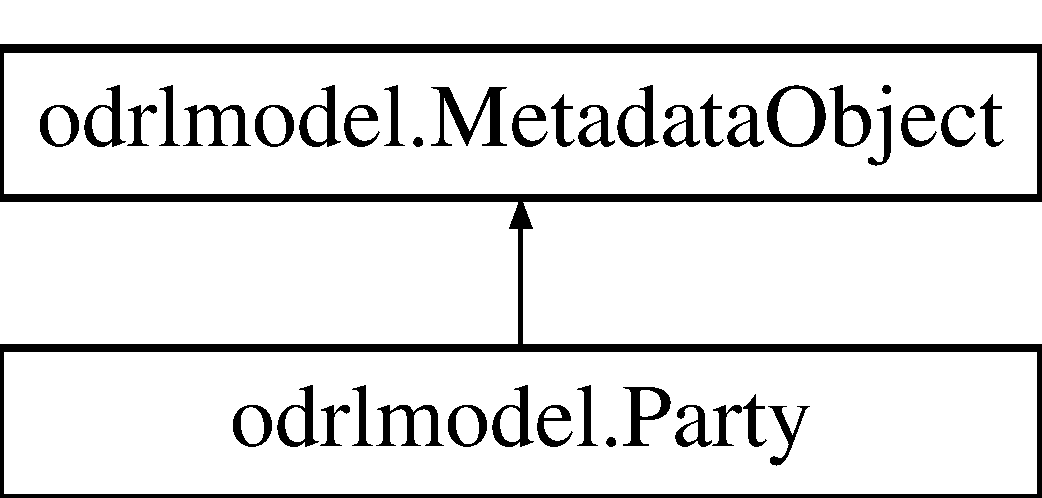
\includegraphics[height=2.000000cm]{classodrlmodel_1_1_party}
\end{center}
\end{figure}
\subsection*{Public Member Functions}
\begin{DoxyCompactItemize}
\item 
\hyperlink{classodrlmodel_1_1_party_a8625ab95a1c49e20d7d9881c0712cbd3}{Party} ()
\item 
\hyperlink{classodrlmodel_1_1_party_a4ac7aad2d6c9d3e5311799432bf59e02}{Party} (\hyperlink{classodrlmodel_1_1_party}{Party} a)
\item 
\hyperlink{classodrlmodel_1_1_party_adcc45332781273d7910daa6cb66a6be1}{Party} (String \-\_\-uri)
\end{DoxyCompactItemize}
\subsection*{Additional Inherited Members}


\subsection{Detailed Description}
This class represents an O\-D\-R\-L2.\-0 \hyperlink{classodrlmodel_1_1_party}{Party} The \hyperlink{classodrlmodel_1_1_party}{Party} entity is aimed at identifying a person, group of people, or organisation. The \hyperlink{classodrlmodel_1_1_party}{Party} M\-U\-S\-T identify a (legal) entity that can participate in policy transactions \begin{DoxyAuthor}{Author}
Victor 
\end{DoxyAuthor}


\subsection{Constructor \& Destructor Documentation}
\hypertarget{classodrlmodel_1_1_party_a8625ab95a1c49e20d7d9881c0712cbd3}{\index{odrlmodel\-::\-Party@{odrlmodel\-::\-Party}!Party@{Party}}
\index{Party@{Party}!odrlmodel::Party@{odrlmodel\-::\-Party}}
\subsubsection[{Party}]{\setlength{\rightskip}{0pt plus 5cm}odrlmodel.\-Party.\-Party (
\begin{DoxyParamCaption}
{}
\end{DoxyParamCaption}
)}}\label{classodrlmodel_1_1_party_a8625ab95a1c49e20d7d9881c0712cbd3}
\hyperlink{classodrlmodel_1_1_party}{Party} constructor with a random U\-R\-I in the default namespace. By default, an party will be like this\-: \href{http://salonica.dia.fi.upm.es/ldr/party/2e7de960-7001-4c07-bde5-c5ad1f35133d}{\tt http\-://salonica.\-dia.\-fi.\-upm.\-es/ldr/party/2e7de960-\/7001-\/4c07-\/bde5-\/c5ad1f35133d} \hypertarget{classodrlmodel_1_1_party_a4ac7aad2d6c9d3e5311799432bf59e02}{\index{odrlmodel\-::\-Party@{odrlmodel\-::\-Party}!Party@{Party}}
\index{Party@{Party}!odrlmodel::Party@{odrlmodel\-::\-Party}}
\subsubsection[{Party}]{\setlength{\rightskip}{0pt plus 5cm}odrlmodel.\-Party.\-Party (
\begin{DoxyParamCaption}
\item[{{\bf Party}}]{a}
\end{DoxyParamCaption}
)}}\label{classodrlmodel_1_1_party_a4ac7aad2d6c9d3e5311799432bf59e02}
Cloner constructor \hypertarget{classodrlmodel_1_1_party_adcc45332781273d7910daa6cb66a6be1}{\index{odrlmodel\-::\-Party@{odrlmodel\-::\-Party}!Party@{Party}}
\index{Party@{Party}!odrlmodel::Party@{odrlmodel\-::\-Party}}
\subsubsection[{Party}]{\setlength{\rightskip}{0pt plus 5cm}odrlmodel.\-Party.\-Party (
\begin{DoxyParamCaption}
\item[{String}]{\-\_\-uri}
\end{DoxyParamCaption}
)}}\label{classodrlmodel_1_1_party_adcc45332781273d7910daa6cb66a6be1}
Creates an party identified by the given U\-R\-I. This \hyperlink{classodrlmodel_1_1_party}{Party} might be one of those defined by O\-D\-R\-L, in which case label, comment, and see\-Also are loaded from the O\-D\-R\-L ontology 
\begin{DoxyParams}{Parameters}
{\em \-\_\-uri} & U\-R\-I of the party \\
\hline
\end{DoxyParams}


The documentation for this class was generated from the following file\-:\begin{DoxyCompactItemize}
\item 
src/odrlmodel/Party.\-java\end{DoxyCompactItemize}

\hypertarget{classodrlmodel_1_1_permission}{\section{odrlmodel.\-Permission Class Reference}
\label{classodrlmodel_1_1_permission}\index{odrlmodel.\-Permission@{odrlmodel.\-Permission}}
}
Inheritance diagram for odrlmodel.\-Permission\-:\begin{figure}[H]
\begin{center}
\leavevmode
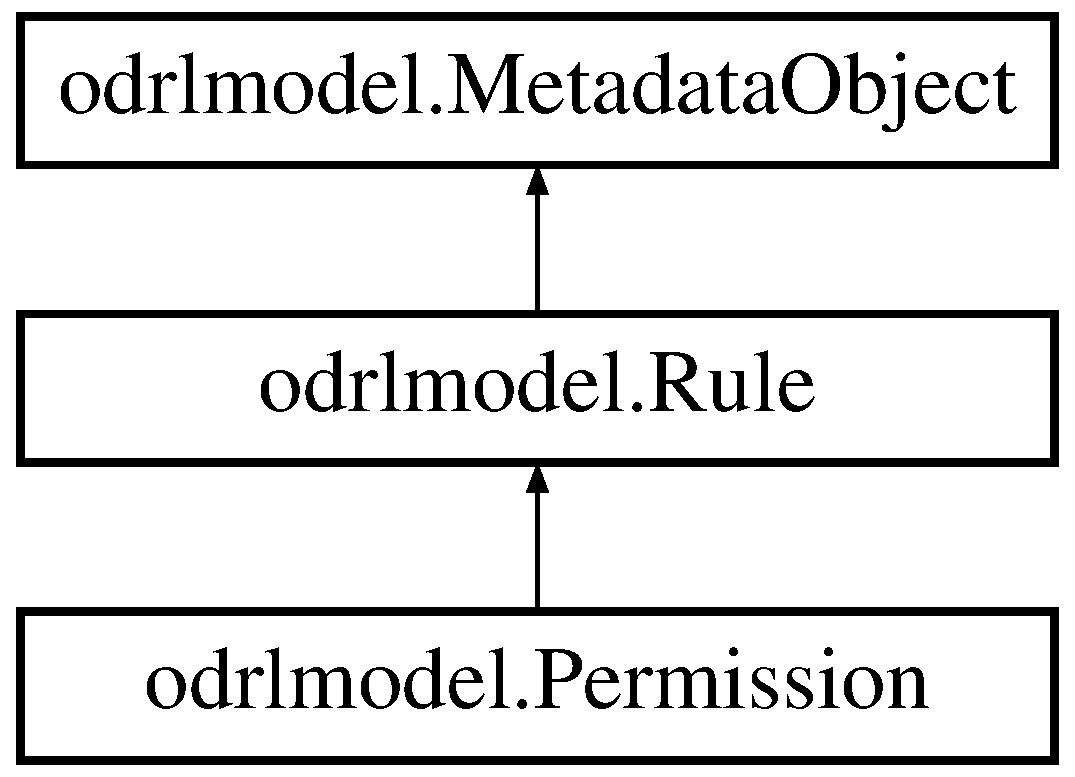
\includegraphics[height=3.000000cm]{classodrlmodel_1_1_permission}
\end{center}
\end{figure}
\subsection*{Public Member Functions}
\begin{DoxyCompactItemize}
\item 
\hyperlink{classodrlmodel_1_1_permission_ac5e432bdda9d75997a93c22fb7d53091}{Permission} ()
\item 
\hyperlink{classodrlmodel_1_1_permission_a28aa45d6c1aa9ad63ec4e7ce43a14a7b}{Permission} (String \-\_\-uri)
\item 
void \hyperlink{classodrlmodel_1_1_permission_a9424e5529df4b49a28a882bd19eb2176}{set\-Duty} (\hyperlink{classodrlmodel_1_1_duty}{Duty} duty)
\item 
void \hyperlink{classodrlmodel_1_1_permission_ac239fbe0c792b3cfe74a2765e5f72a21}{set\-Duties} (List$<$ \hyperlink{classodrlmodel_1_1_duty}{Duty} $>$ \-\_\-duties)
\item 
List$<$ \hyperlink{classodrlmodel_1_1_duty}{Duty} $>$ \hyperlink{classodrlmodel_1_1_permission_a10e8e0171aadc06457192b15cd12bc00}{get\-Duties} ()
\end{DoxyCompactItemize}
\subsection*{Additional Inherited Members}


\subsection{Detailed Description}
The \hyperlink{classodrlmodel_1_1_permission}{Permission} entity indicates the Actions that the assignee is permitted to perform on the associated \hyperlink{classodrlmodel_1_1_asset}{Asset}. In other words, what the assigner (supplier) has granted to the assignee (consumer).

An O\-D\-R\-L policy expression M\-A\-Y contain at least one \hyperlink{classodrlmodel_1_1_permission}{Permission}. It is important to verify the semantics of the \hyperlink{classodrlmodel_1_1_policy}{Policy} type attribute as this M\-A\-Y indicate additional constraints on the \hyperlink{classodrlmodel_1_1_policy}{Policy} expression structure.

If several \hyperlink{classodrlmodel_1_1_permission}{Permission} entities are referred to by a \hyperlink{classodrlmodel_1_1_policy}{Policy}, then all of them are valid.

\begin{DoxyAuthor}{Author}
Victor Rodriguez Doncel at O\-E\-G-\/\-U\-P\-M 2014 
\end{DoxyAuthor}


\subsection{Constructor \& Destructor Documentation}
\hypertarget{classodrlmodel_1_1_permission_ac5e432bdda9d75997a93c22fb7d53091}{\index{odrlmodel\-::\-Permission@{odrlmodel\-::\-Permission}!Permission@{Permission}}
\index{Permission@{Permission}!odrlmodel::Permission@{odrlmodel\-::\-Permission}}
\subsubsection[{Permission}]{\setlength{\rightskip}{0pt plus 5cm}odrlmodel.\-Permission.\-Permission (
\begin{DoxyParamCaption}
{}
\end{DoxyParamCaption}
)}}\label{classodrlmodel_1_1_permission_ac5e432bdda9d75997a93c22fb7d53091}
\hyperlink{classodrlmodel_1_1_permission}{Permission} constructor \hyperlink{classodrlmodel_1_1_permission}{Permission} are by default anonymous \hypertarget{classodrlmodel_1_1_permission_a28aa45d6c1aa9ad63ec4e7ce43a14a7b}{\index{odrlmodel\-::\-Permission@{odrlmodel\-::\-Permission}!Permission@{Permission}}
\index{Permission@{Permission}!odrlmodel::Permission@{odrlmodel\-::\-Permission}}
\subsubsection[{Permission}]{\setlength{\rightskip}{0pt plus 5cm}odrlmodel.\-Permission.\-Permission (
\begin{DoxyParamCaption}
\item[{String}]{\-\_\-uri}
\end{DoxyParamCaption}
)}}\label{classodrlmodel_1_1_permission_a28aa45d6c1aa9ad63ec4e7ce43a14a7b}
Creates a permission identified by the given U\-R\-I. 
\begin{DoxyParams}{Parameters}
{\em \-\_\-uri} & U\-R\-I of the prohibition \\
\hline
\end{DoxyParams}


\subsection{Member Function Documentation}
\hypertarget{classodrlmodel_1_1_permission_a10e8e0171aadc06457192b15cd12bc00}{\index{odrlmodel\-::\-Permission@{odrlmodel\-::\-Permission}!get\-Duties@{get\-Duties}}
\index{get\-Duties@{get\-Duties}!odrlmodel::Permission@{odrlmodel\-::\-Permission}}
\subsubsection[{get\-Duties}]{\setlength{\rightskip}{0pt plus 5cm}List$<${\bf Duty}$>$ odrlmodel.\-Permission.\-get\-Duties (
\begin{DoxyParamCaption}
{}
\end{DoxyParamCaption}
)}}\label{classodrlmodel_1_1_permission_a10e8e0171aadc06457192b15cd12bc00}
Sets the duties associated to this permission \begin{DoxyReturn}{Returns}
List of duties 
\end{DoxyReturn}
\hypertarget{classodrlmodel_1_1_permission_ac239fbe0c792b3cfe74a2765e5f72a21}{\index{odrlmodel\-::\-Permission@{odrlmodel\-::\-Permission}!set\-Duties@{set\-Duties}}
\index{set\-Duties@{set\-Duties}!odrlmodel::Permission@{odrlmodel\-::\-Permission}}
\subsubsection[{set\-Duties}]{\setlength{\rightskip}{0pt plus 5cm}void odrlmodel.\-Permission.\-set\-Duties (
\begin{DoxyParamCaption}
\item[{List$<$ {\bf Duty} $>$}]{\-\_\-duties}
\end{DoxyParamCaption}
)}}\label{classodrlmodel_1_1_permission_ac239fbe0c792b3cfe74a2765e5f72a21}
Sets the duties associated to this permission 
\begin{DoxyParams}{Parameters}
{\em \-\_\-duties} & List of duties to be retrieved \\
\hline
\end{DoxyParams}
\hypertarget{classodrlmodel_1_1_permission_a9424e5529df4b49a28a882bd19eb2176}{\index{odrlmodel\-::\-Permission@{odrlmodel\-::\-Permission}!set\-Duty@{set\-Duty}}
\index{set\-Duty@{set\-Duty}!odrlmodel::Permission@{odrlmodel\-::\-Permission}}
\subsubsection[{set\-Duty}]{\setlength{\rightskip}{0pt plus 5cm}void odrlmodel.\-Permission.\-set\-Duty (
\begin{DoxyParamCaption}
\item[{{\bf Duty}}]{duty}
\end{DoxyParamCaption}
)}}\label{classodrlmodel_1_1_permission_a9424e5529df4b49a28a882bd19eb2176}
Sets a single duty associated to this permission 
\begin{DoxyParams}{Parameters}
{\em duty} & \hyperlink{classodrlmodel_1_1_duty}{Duty} to be retrieved \\
\hline
\end{DoxyParams}


The documentation for this class was generated from the following file\-:\begin{DoxyCompactItemize}
\item 
src/odrlmodel/Permission.\-java\end{DoxyCompactItemize}

\hypertarget{classodrlmodel_1_1_policy}{\section{odrlmodel.\-Policy Class Reference}
\label{classodrlmodel_1_1_policy}\index{odrlmodel.\-Policy@{odrlmodel.\-Policy}}
}
Inheritance diagram for odrlmodel.\-Policy\-:\begin{figure}[H]
\begin{center}
\leavevmode
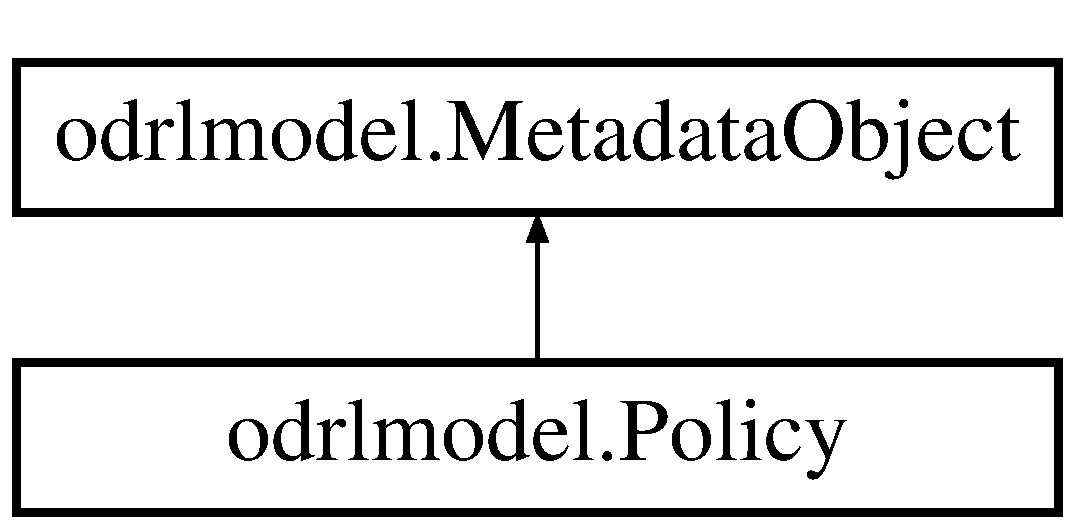
\includegraphics[height=2.000000cm]{classodrlmodel_1_1_policy}
\end{center}
\end{figure}
\subsection*{Public Member Functions}
\begin{DoxyCompactItemize}
\item 
\hyperlink{classodrlmodel_1_1_policy_aa9b13e9353f711831ebedfd0aae45872}{Policy} ()
\item 
\hyperlink{classodrlmodel_1_1_policy_aebe74ea9719b1d43c650964f1ec6b7fb}{Policy} (String \-\_\-uri)
\item 
int \hyperlink{classodrlmodel_1_1_policy_a288746977d9b84e16ba7db3e1dda4068}{get\-Type} ()
\item 
void \hyperlink{classodrlmodel_1_1_policy_a4c74f621b29d742f9df45a9bf0c95826}{set\-Type} (int \-\_\-type)
\item 
void \hyperlink{classodrlmodel_1_1_policy_a8100fcce6e529bcb638698274209a7ab}{add\-Rule} (\hyperlink{classodrlmodel_1_1_rule}{Rule} r)
\item 
List$<$ \hyperlink{classodrlmodel_1_1_rule}{Rule} $>$ \hyperlink{classodrlmodel_1_1_policy_a112aa1e5e6afcbd40ddc4db602a19edf}{get\-Rules} ()
\item 
void \hyperlink{classodrlmodel_1_1_policy_a04cf98a54bb431b372a1603115c6b590}{set\-Rules} (List$<$ \hyperlink{classodrlmodel_1_1_rule}{Rule} $>$ \-\_\-rules)
\item 
void \hyperlink{classodrlmodel_1_1_policy_ab7f7e6cb828a4ab801b1641742d90446}{set\-Target\-In\-All\-Rules} (String target\-Name)
\item 
void \hyperlink{classodrlmodel_1_1_policy_a2cbd861f16cd8c942f5905d2b64dc836}{set\-Assignee\-In\-All\-Rules} (\hyperlink{classodrlmodel_1_1_party}{Party} assignee)
\item 
void \hyperlink{classodrlmodel_1_1_policy_a5db6c01f28698efbc325763bd93ad265}{set\-Assigner\-In\-All\-Rules} (\hyperlink{classodrlmodel_1_1_party}{Party} assigner)
\end{DoxyCompactItemize}
\subsection*{Static Public Attributes}
\begin{DoxyCompactItemize}
\item 
\hypertarget{classodrlmodel_1_1_policy_ac21b03b084083baf13c68ae71cceabad}{static final int {\bfseries P\-O\-L\-I\-C\-Y\-\_\-\-S\-E\-T} = 0}\label{classodrlmodel_1_1_policy_ac21b03b084083baf13c68ae71cceabad}

\item 
\hypertarget{classodrlmodel_1_1_policy_ad9764f12c73e051fc961e2962a42e107}{static final int {\bfseries P\-O\-L\-I\-C\-Y\-\_\-\-R\-E\-Q\-U\-E\-S\-T} = 1}\label{classodrlmodel_1_1_policy_ad9764f12c73e051fc961e2962a42e107}

\item 
\hypertarget{classodrlmodel_1_1_policy_aea7a829bafc34b98a72cd344b8285bcc}{static final int {\bfseries P\-O\-L\-I\-C\-Y\-\_\-\-O\-F\-F\-E\-R} = 2}\label{classodrlmodel_1_1_policy_aea7a829bafc34b98a72cd344b8285bcc}

\item 
\hypertarget{classodrlmodel_1_1_policy_a0d7c3db4e146f25bf30b684efc962f18}{static final int {\bfseries P\-O\-L\-I\-C\-Y\-\_\-\-C\-C} = 3}\label{classodrlmodel_1_1_policy_a0d7c3db4e146f25bf30b684efc962f18}

\item 
\hypertarget{classodrlmodel_1_1_policy_ae11df1da254f43aae6418d0a71723103}{static final int {\bfseries P\-O\-L\-I\-C\-Y\-\_\-\-A\-G\-R\-E\-E\-M\-E\-N\-T} = 4}\label{classodrlmodel_1_1_policy_ae11df1da254f43aae6418d0a71723103}

\item 
\hypertarget{classodrlmodel_1_1_policy_a9c0b3d10c39931b9bb4f3656055b12e7}{static final int {\bfseries P\-O\-L\-I\-C\-Y\-\_\-\-T\-I\-C\-K\-E\-T} = 5}\label{classodrlmodel_1_1_policy_a9c0b3d10c39931b9bb4f3656055b12e7}

\end{DoxyCompactItemize}
\subsection*{Protected Attributes}
\begin{DoxyCompactItemize}
\item 
\hypertarget{classodrlmodel_1_1_policy_a78dc893b4b6be02dc15022f67431d9d4}{List$<$ \hyperlink{classodrlmodel_1_1_rule}{Rule} $>$ {\bfseries rules} = new Array\-List()}\label{classodrlmodel_1_1_policy_a78dc893b4b6be02dc15022f67431d9d4}

\item 
\hypertarget{classodrlmodel_1_1_policy_a2ee78152028a84149c0099df7d9e3d64}{String {\bfseries file\-Name} = \char`\"{}\char`\"{}}\label{classodrlmodel_1_1_policy_a2ee78152028a84149c0099df7d9e3d64}

\end{DoxyCompactItemize}
\subsection*{Additional Inherited Members}


\subsection{Detailed Description}
\hyperlink{classodrlmodel_1_1_policy}{Policy} represents an O\-D\-R\-L policy, supporting a reduced set of the features defined in the O\-D\-R\-L2.\-0 specification

The \hyperlink{classodrlmodel_1_1_policy}{Policy} entity is the top-\/level entity.

An abstract common ancestor to Permissions, Prohibitions and Duties.  For more information, check \href{http://www.w3.org/community/odrl/two/model/#section-21}{\tt http\-://www.\-w3.\-org/community/odrl/two/model/\#section-\/21} \begin{DoxyAuthor}{Author}
Victor Rodriguez Doncel at O\-E\-G-\/\-U\-P\-M 2014 
\end{DoxyAuthor}


\subsection{Constructor \& Destructor Documentation}
\hypertarget{classodrlmodel_1_1_policy_aa9b13e9353f711831ebedfd0aae45872}{\index{odrlmodel\-::\-Policy@{odrlmodel\-::\-Policy}!Policy@{Policy}}
\index{Policy@{Policy}!odrlmodel::Policy@{odrlmodel\-::\-Policy}}
\subsubsection[{Policy}]{\setlength{\rightskip}{0pt plus 5cm}odrlmodel.\-Policy.\-Policy (
\begin{DoxyParamCaption}
{}
\end{DoxyParamCaption}
)}}\label{classodrlmodel_1_1_policy_aa9b13e9353f711831ebedfd0aae45872}
\hyperlink{classodrlmodel_1_1_policy}{Policy} constructor with a random U\-R\-I in the default namespace A policy is by default a Set policy \hypertarget{classodrlmodel_1_1_policy_aebe74ea9719b1d43c650964f1ec6b7fb}{\index{odrlmodel\-::\-Policy@{odrlmodel\-::\-Policy}!Policy@{Policy}}
\index{Policy@{Policy}!odrlmodel::Policy@{odrlmodel\-::\-Policy}}
\subsubsection[{Policy}]{\setlength{\rightskip}{0pt plus 5cm}odrlmodel.\-Policy.\-Policy (
\begin{DoxyParamCaption}
\item[{String}]{\-\_\-uri}
\end{DoxyParamCaption}
)}}\label{classodrlmodel_1_1_policy_aebe74ea9719b1d43c650964f1ec6b7fb}
\hyperlink{classodrlmodel_1_1_policy}{Policy} constructor with a given U\-R\-I A policy is by default a Set policy 
\begin{DoxyParams}{Parameters}
{\em \-\_\-uri} & Given U\-R\-I \\
\hline
\end{DoxyParams}


\subsection{Member Function Documentation}
\hypertarget{classodrlmodel_1_1_policy_a8100fcce6e529bcb638698274209a7ab}{\index{odrlmodel\-::\-Policy@{odrlmodel\-::\-Policy}!add\-Rule@{add\-Rule}}
\index{add\-Rule@{add\-Rule}!odrlmodel::Policy@{odrlmodel\-::\-Policy}}
\subsubsection[{add\-Rule}]{\setlength{\rightskip}{0pt plus 5cm}void odrlmodel.\-Policy.\-add\-Rule (
\begin{DoxyParamCaption}
\item[{{\bf Rule}}]{r}
\end{DoxyParamCaption}
)}}\label{classodrlmodel_1_1_policy_a8100fcce6e529bcb638698274209a7ab}
Adds a rule to the policy 
\begin{DoxyParams}{Parameters}
{\em r} & \hyperlink{classodrlmodel_1_1_rule}{Rule} to be added \\
\hline
\end{DoxyParams}
\hypertarget{classodrlmodel_1_1_policy_a112aa1e5e6afcbd40ddc4db602a19edf}{\index{odrlmodel\-::\-Policy@{odrlmodel\-::\-Policy}!get\-Rules@{get\-Rules}}
\index{get\-Rules@{get\-Rules}!odrlmodel::Policy@{odrlmodel\-::\-Policy}}
\subsubsection[{get\-Rules}]{\setlength{\rightskip}{0pt plus 5cm}List$<${\bf Rule}$>$ odrlmodel.\-Policy.\-get\-Rules (
\begin{DoxyParamCaption}
{}
\end{DoxyParamCaption}
)}}\label{classodrlmodel_1_1_policy_a112aa1e5e6afcbd40ddc4db602a19edf}
Gets the list of rules this policy has \begin{DoxyReturn}{Returns}
List of rules 
\end{DoxyReturn}
\hypertarget{classodrlmodel_1_1_policy_a288746977d9b84e16ba7db3e1dda4068}{\index{odrlmodel\-::\-Policy@{odrlmodel\-::\-Policy}!get\-Type@{get\-Type}}
\index{get\-Type@{get\-Type}!odrlmodel::Policy@{odrlmodel\-::\-Policy}}
\subsubsection[{get\-Type}]{\setlength{\rightskip}{0pt plus 5cm}int odrlmodel.\-Policy.\-get\-Type (
\begin{DoxyParamCaption}
{}
\end{DoxyParamCaption}
)}}\label{classodrlmodel_1_1_policy_a288746977d9b84e16ba7db3e1dda4068}
Gets the type of the \hyperlink{classodrlmodel_1_1_policy}{Policy} \begin{DoxyReturn}{Returns}
one of\-: Policy.\-P\-O\-L\-I\-C\-Y\-\_\-\-S\-E\-T, Policy.\-P\-O\-L\-I\-C\-Y\-\_\-\-R\-E\-Q\-U\-E\-S\-T, Policy.\-P\-O\-L\-I\-C\-Y\-\_\-\-O\-F\-F\-E\-R 
\end{DoxyReturn}
\hypertarget{classodrlmodel_1_1_policy_a2cbd861f16cd8c942f5905d2b64dc836}{\index{odrlmodel\-::\-Policy@{odrlmodel\-::\-Policy}!set\-Assignee\-In\-All\-Rules@{set\-Assignee\-In\-All\-Rules}}
\index{set\-Assignee\-In\-All\-Rules@{set\-Assignee\-In\-All\-Rules}!odrlmodel::Policy@{odrlmodel\-::\-Policy}}
\subsubsection[{set\-Assignee\-In\-All\-Rules}]{\setlength{\rightskip}{0pt plus 5cm}void odrlmodel.\-Policy.\-set\-Assignee\-In\-All\-Rules (
\begin{DoxyParamCaption}
\item[{{\bf Party}}]{assignee}
\end{DoxyParamCaption}
)}}\label{classodrlmodel_1_1_policy_a2cbd861f16cd8c942f5905d2b64dc836}
Sets a certain assignee in all the rules 
\begin{DoxyParams}{Parameters}
{\em assignee} & \hyperlink{classodrlmodel_1_1_party}{Party} assigner \\
\hline
\end{DoxyParams}
\hypertarget{classodrlmodel_1_1_policy_a5db6c01f28698efbc325763bd93ad265}{\index{odrlmodel\-::\-Policy@{odrlmodel\-::\-Policy}!set\-Assigner\-In\-All\-Rules@{set\-Assigner\-In\-All\-Rules}}
\index{set\-Assigner\-In\-All\-Rules@{set\-Assigner\-In\-All\-Rules}!odrlmodel::Policy@{odrlmodel\-::\-Policy}}
\subsubsection[{set\-Assigner\-In\-All\-Rules}]{\setlength{\rightskip}{0pt plus 5cm}void odrlmodel.\-Policy.\-set\-Assigner\-In\-All\-Rules (
\begin{DoxyParamCaption}
\item[{{\bf Party}}]{assigner}
\end{DoxyParamCaption}
)}}\label{classodrlmodel_1_1_policy_a5db6c01f28698efbc325763bd93ad265}
Sets a certain assigner in all the rules 
\begin{DoxyParams}{Parameters}
{\em assigner} & \hyperlink{classodrlmodel_1_1_party}{Party} assigner \\
\hline
\end{DoxyParams}
\hypertarget{classodrlmodel_1_1_policy_a04cf98a54bb431b372a1603115c6b590}{\index{odrlmodel\-::\-Policy@{odrlmodel\-::\-Policy}!set\-Rules@{set\-Rules}}
\index{set\-Rules@{set\-Rules}!odrlmodel::Policy@{odrlmodel\-::\-Policy}}
\subsubsection[{set\-Rules}]{\setlength{\rightskip}{0pt plus 5cm}void odrlmodel.\-Policy.\-set\-Rules (
\begin{DoxyParamCaption}
\item[{List$<$ {\bf Rule} $>$}]{\-\_\-rules}
\end{DoxyParamCaption}
)}}\label{classodrlmodel_1_1_policy_a04cf98a54bb431b372a1603115c6b590}
Sets the list of rules 
\begin{DoxyParams}{Parameters}
{\em \-\_\-rules} & List of rules \\
\hline
\end{DoxyParams}
\hypertarget{classodrlmodel_1_1_policy_ab7f7e6cb828a4ab801b1641742d90446}{\index{odrlmodel\-::\-Policy@{odrlmodel\-::\-Policy}!set\-Target\-In\-All\-Rules@{set\-Target\-In\-All\-Rules}}
\index{set\-Target\-In\-All\-Rules@{set\-Target\-In\-All\-Rules}!odrlmodel::Policy@{odrlmodel\-::\-Policy}}
\subsubsection[{set\-Target\-In\-All\-Rules}]{\setlength{\rightskip}{0pt plus 5cm}void odrlmodel.\-Policy.\-set\-Target\-In\-All\-Rules (
\begin{DoxyParamCaption}
\item[{String}]{target\-Name}
\end{DoxyParamCaption}
)}}\label{classodrlmodel_1_1_policy_ab7f7e6cb828a4ab801b1641742d90446}
Sets a certain target in all the rules 
\begin{DoxyParams}{Parameters}
{\em target\-Name} & Name of the target \\
\hline
\end{DoxyParams}
\hypertarget{classodrlmodel_1_1_policy_a4c74f621b29d742f9df45a9bf0c95826}{\index{odrlmodel\-::\-Policy@{odrlmodel\-::\-Policy}!set\-Type@{set\-Type}}
\index{set\-Type@{set\-Type}!odrlmodel::Policy@{odrlmodel\-::\-Policy}}
\subsubsection[{set\-Type}]{\setlength{\rightskip}{0pt plus 5cm}void odrlmodel.\-Policy.\-set\-Type (
\begin{DoxyParamCaption}
\item[{int}]{\-\_\-type}
\end{DoxyParamCaption}
)}}\label{classodrlmodel_1_1_policy_a4c74f621b29d742f9df45a9bf0c95826}
Sets the type of the policy 
\begin{DoxyParams}{Parameters}
{\em \-\_\-type,one} & of\-: Policy.\-P\-O\-L\-I\-C\-Y\-\_\-\-S\-E\-T, Policy.\-P\-O\-L\-I\-C\-Y\-\_\-\-R\-E\-Q\-U\-E\-S\-T, Policy.\-P\-O\-L\-I\-C\-Y\-\_\-\-O\-F\-F\-E\-R \\
\hline
\end{DoxyParams}


The documentation for this class was generated from the following file\-:\begin{DoxyCompactItemize}
\item 
src/odrlmodel/Policy.\-java\end{DoxyCompactItemize}

\hypertarget{classodrlmodel_1_1_prohibition}{\section{odrlmodel.\-Prohibition Class Reference}
\label{classodrlmodel_1_1_prohibition}\index{odrlmodel.\-Prohibition@{odrlmodel.\-Prohibition}}
}
Inheritance diagram for odrlmodel.\-Prohibition\-:\begin{figure}[H]
\begin{center}
\leavevmode
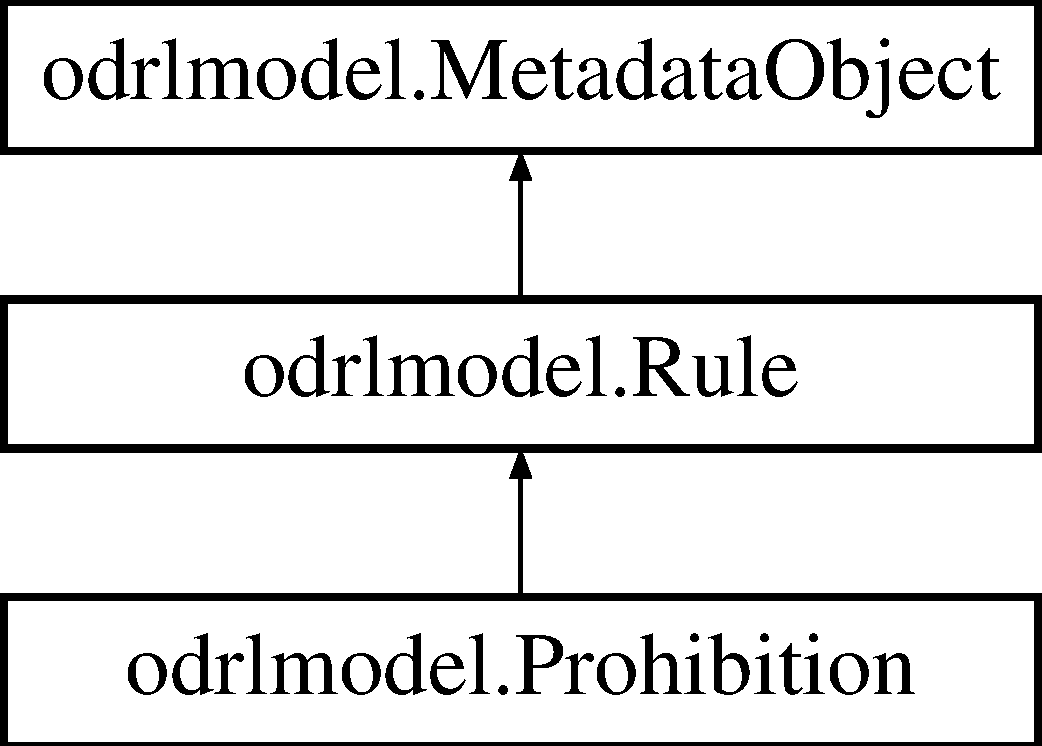
\includegraphics[height=3.000000cm]{classodrlmodel_1_1_prohibition}
\end{center}
\end{figure}
\subsection*{Public Member Functions}
\begin{DoxyCompactItemize}
\item 
\hyperlink{classodrlmodel_1_1_prohibition_a444002a7ca9513c35688bac18f176b0a}{Prohibition} ()
\item 
\hyperlink{classodrlmodel_1_1_prohibition_aa76b9833e97cd020ef8bf27469b39da6}{Prohibition} (String \-\_\-uri)
\end{DoxyCompactItemize}
\subsection*{Additional Inherited Members}


\subsection{Detailed Description}
Represents an O\-D\-R\-L2.\-0 \hyperlink{classodrlmodel_1_1_prohibition}{Prohibition}.

The \hyperlink{classodrlmodel_1_1_prohibition}{Prohibition} entity indicates the Actions that the assignee is prohibited to perform on the related \hyperlink{classodrlmodel_1_1_asset}{Asset} \mbox{[}O\-D\-R\-L-\/\-R\-E\-Q-\/1.\-7\mbox{]}. Prohibitions are issued by the supplier of the \hyperlink{classodrlmodel_1_1_asset}{Asset} – the \hyperlink{classodrlmodel_1_1_party}{Party} with the Role assigner. If several \hyperlink{classodrlmodel_1_1_prohibition}{Prohibition} entities are referred to by a \hyperlink{classodrlmodel_1_1_policy}{Policy}, all of them are valid.

\begin{DoxyAuthor}{Author}
Victor 
\end{DoxyAuthor}


\subsection{Constructor \& Destructor Documentation}
\hypertarget{classodrlmodel_1_1_prohibition_a444002a7ca9513c35688bac18f176b0a}{\index{odrlmodel\-::\-Prohibition@{odrlmodel\-::\-Prohibition}!Prohibition@{Prohibition}}
\index{Prohibition@{Prohibition}!odrlmodel::Prohibition@{odrlmodel\-::\-Prohibition}}
\subsubsection[{Prohibition}]{\setlength{\rightskip}{0pt plus 5cm}odrlmodel.\-Prohibition.\-Prohibition (
\begin{DoxyParamCaption}
{}
\end{DoxyParamCaption}
)}}\label{classodrlmodel_1_1_prohibition_a444002a7ca9513c35688bac18f176b0a}
\hyperlink{classodrlmodel_1_1_prohibition}{Prohibition} constructor Prohibitions are by default anonymous \hypertarget{classodrlmodel_1_1_prohibition_aa76b9833e97cd020ef8bf27469b39da6}{\index{odrlmodel\-::\-Prohibition@{odrlmodel\-::\-Prohibition}!Prohibition@{Prohibition}}
\index{Prohibition@{Prohibition}!odrlmodel::Prohibition@{odrlmodel\-::\-Prohibition}}
\subsubsection[{Prohibition}]{\setlength{\rightskip}{0pt plus 5cm}odrlmodel.\-Prohibition.\-Prohibition (
\begin{DoxyParamCaption}
\item[{String}]{\-\_\-uri}
\end{DoxyParamCaption}
)}}\label{classodrlmodel_1_1_prohibition_aa76b9833e97cd020ef8bf27469b39da6}
Creates a prohibition identified by the given U\-R\-I. 
\begin{DoxyParams}{Parameters}
{\em \-\_\-uri} & U\-R\-I of the prohibition \\
\hline
\end{DoxyParams}


The documentation for this class was generated from the following file\-:\begin{DoxyCompactItemize}
\item 
src/odrlmodel/Prohibition.\-java\end{DoxyCompactItemize}

\hypertarget{classodrlmodel_1_1_r_d_f_utils}{\section{odrlmodel.\-R\-D\-F\-Utils Class Reference}
\label{classodrlmodel_1_1_r_d_f_utils}\index{odrlmodel.\-R\-D\-F\-Utils@{odrlmodel.\-R\-D\-F\-Utils}}
}
\subsection*{Public Member Functions}
\begin{DoxyCompactItemize}
\item 
\hypertarget{classodrlmodel_1_1_r_d_f_utils_af022181a14e893d47069a2c000610ac3}{String {\bfseries to\-String} ()}\label{classodrlmodel_1_1_r_d_f_utils_af022181a14e893d47069a2c000610ac3}

\end{DoxyCompactItemize}
\subsection*{Static Public Member Functions}
\begin{DoxyCompactItemize}
\item 
static List$<$ String $>$ \hyperlink{classodrlmodel_1_1_r_d_f_utils_aa5ba71deae00f5e6fdf2019989c992ed}{get\-Core\-O\-D\-R\-L\-Actions} ()
\item 
\hypertarget{classodrlmodel_1_1_r_d_f_utils_aabe3570587849c1b57a8d6def3170c7d}{static String {\bfseries get\-Individual\-Label} (String uri)}\label{classodrlmodel_1_1_r_d_f_utils_aabe3570587849c1b57a8d6def3170c7d}

\item 
\hypertarget{classodrlmodel_1_1_r_d_f_utils_a72e3fc78f978e61fad2914802d0e2cdb}{static String {\bfseries get\-Individual\-Comment} (String uri)}\label{classodrlmodel_1_1_r_d_f_utils_a72e3fc78f978e61fad2914802d0e2cdb}

\item 
static \hyperlink{classodrlmodel_1_1_action}{Action} \hyperlink{classodrlmodel_1_1_r_d_f_utils_a2f50a747438b23a3570e0a9266327e22}{enrich\-Action} (\hyperlink{classodrlmodel_1_1_action}{Action} action1)
\item 
static \hyperlink{classodrlmodel_1_1_constraint}{Constraint} \hyperlink{classodrlmodel_1_1_r_d_f_utils_a9bcd3726b8c1b5445893ec78c40be15e}{enrich\-Constraint} (\hyperlink{classodrlmodel_1_1_constraint}{Constraint} coriginal)
\item 
static List$<$ \hyperlink{classodrlmodel_1_1_action}{Action} $>$ \hyperlink{classodrlmodel_1_1_r_d_f_utils_a7688338085fad38120729dda373eaa49}{get\-Basic\-Actions} ()
\item 
static List$<$ \hyperlink{classodrlmodel_1_1_action}{Action} $>$ \hyperlink{classodrlmodel_1_1_r_d_f_utils_ac659a8fb209fa1afeb06fe9dbaa0ae8e}{get\-Basic\-Duties} ()
\item 
static List$<$ \hyperlink{classodrlmodel_1_1_constraint}{Constraint} $>$ \hyperlink{classodrlmodel_1_1_r_d_f_utils_a157ceb5999c149124ae840b86ab1eeef}{get\-Basic\-Constraints} ()
\item 
\hypertarget{classodrlmodel_1_1_r_d_f_utils_ac4e66a6467849b55a54494602f1b7cf4}{static void {\bfseries print} (Model modelo)}\label{classodrlmodel_1_1_r_d_f_utils_ac4e66a6467849b55a54494602f1b7cf4}

\item 
\hypertarget{classodrlmodel_1_1_r_d_f_utils_a66375620306250accde6e2e4f5b977cc}{static boolean {\bfseries save} (Model modelo, String filename)}\label{classodrlmodel_1_1_r_d_f_utils_a66375620306250accde6e2e4f5b977cc}

\item 
\hypertarget{classodrlmodel_1_1_r_d_f_utils_afa67328ddc30751b2ec763cfa96c6656}{static boolean {\bfseries save} (String modelo, String filename)}\label{classodrlmodel_1_1_r_d_f_utils_afa67328ddc30751b2ec763cfa96c6656}

\item 
static \hyperlink{classodrlmodel_1_1_rule}{Rule} \hyperlink{classodrlmodel_1_1_r_d_f_utils_a6d5c9c89380bd3acd24146ba5d606c2d}{find\-Creative\-Commons} (Resource rpolicy)
\item 
static List$<$ Resource $>$ \hyperlink{classodrlmodel_1_1_r_d_f_utils_abefc86cbe6d583263d886dced6270c26}{get\-Ont\-Resources\-Of\-Type} (Model model, Resource resource)
\item 
static List$<$ Resource $>$ \hyperlink{classodrlmodel_1_1_r_d_f_utils_a20fbbdb205c54764d7992b435c160683}{get\-Resources\-Of\-Type} (Model model, Resource resource)
\item 
static List$<$ String $>$ \hyperlink{classodrlmodel_1_1_r_d_f_utils_a53b83408867f19677312116d888cfacb}{get\-Objects\-Of\-Type} (Model model, Resource resource)
\item 
\hypertarget{classodrlmodel_1_1_r_d_f_utils_a238265d7601a0db59f324ab8212b33a2}{static List$<$ String $>$ {\bfseries get\-Objects\-Of\-Type} (Model model, String uri)}\label{classodrlmodel_1_1_r_d_f_utils_a238265d7601a0db59f324ab8212b33a2}

\item 
static String \hyperlink{classodrlmodel_1_1_r_d_f_utils_a92339438ffa0a28247f1f1b0427bb5a6}{get\-First\-Property\-Value} (Resource resource, Property property)
\item 
static List$<$ String $>$ \hyperlink{classodrlmodel_1_1_r_d_f_utils_a7050cd7280dcf28585463eddb174180e}{get\-All\-Property\-Strings} (Resource resource, Property property)
\item 
\hypertarget{classodrlmodel_1_1_r_d_f_utils_a90d0a9bbf8b99e64afe5f1e5fd636fe7}{static List$<$ Resource $>$ {\bfseries get\-All\-Property\-Resources} (Resource resource, Property property)}\label{classodrlmodel_1_1_r_d_f_utils_a90d0a9bbf8b99e64afe5f1e5fd636fe7}

\end{DoxyCompactItemize}
\subsection*{Static Public Attributes}
\begin{DoxyCompactItemize}
\item 
\hypertarget{classodrlmodel_1_1_r_d_f_utils_a095ba20cefe97c59b99f5f62e5241e5d}{static Property {\bfseries T\-I\-T\-L\-E} = Model\-Factory.\-create\-Default\-Model().create\-Property(\char`\"{}http\-://purl.\-org/dc/terms/title\char`\"{})}\label{classodrlmodel_1_1_r_d_f_utils_a095ba20cefe97c59b99f5f62e5241e5d}

\item 
\hypertarget{classodrlmodel_1_1_r_d_f_utils_a6ec492c7244e1ba78dcdbc1a047fff1a}{static Property {\bfseries C\-O\-M\-M\-E\-N\-T} = Model\-Factory.\-create\-Default\-Model().create\-Property(\char`\"{}http\-://www.\-w3.\-org/2000/01/rdf-\/schema\#comment\char`\"{})}\label{classodrlmodel_1_1_r_d_f_utils_a6ec492c7244e1ba78dcdbc1a047fff1a}

\item 
\hypertarget{classodrlmodel_1_1_r_d_f_utils_a0db828183c882c2b564e0f6da42f1d5a}{static Property {\bfseries R\-I\-G\-H\-T\-S} = Model\-Factory.\-create\-Default\-Model().create\-Property(\char`\"{}http\-://purl.\-org/dc/terms/rights\char`\"{})}\label{classodrlmodel_1_1_r_d_f_utils_a0db828183c882c2b564e0f6da42f1d5a}

\item 
\hypertarget{classodrlmodel_1_1_r_d_f_utils_aa2275f5f68d0d27bf845393a3e7c2dd4}{static Property {\bfseries R\-L\-I\-C\-E\-N\-S\-E} = Model\-Factory.\-create\-Default\-Model().create\-Property(\char`\"{}http\-://purl.\-org/dc/terms/license\char`\"{})}\label{classodrlmodel_1_1_r_d_f_utils_aa2275f5f68d0d27bf845393a3e7c2dd4}

\item 
\hypertarget{classodrlmodel_1_1_r_d_f_utils_ae069861fdbfe8ab1b905dd2289fe07bb}{static Property {\bfseries L\-A\-B\-E\-L} = Model\-Factory.\-create\-Default\-Model().create\-Property(\char`\"{}http\-://www.\-w3.\-org/2000/01/rdf-\/schema\#label\char`\"{})}\label{classodrlmodel_1_1_r_d_f_utils_ae069861fdbfe8ab1b905dd2289fe07bb}

\item 
\hypertarget{classodrlmodel_1_1_r_d_f_utils_abed84ce9ab44adf6778df448352c9e09}{static Property {\bfseries S\-E\-E\-A\-L\-S\-O} = Model\-Factory.\-create\-Default\-Model().create\-Property(\char`\"{}http\-://www.\-w3.\-org/2000/01/rdf-\/schema\#see\-Also\char`\"{})}\label{classodrlmodel_1_1_r_d_f_utils_abed84ce9ab44adf6778df448352c9e09}

\item 
\hypertarget{classodrlmodel_1_1_r_d_f_utils_ae28d333f5d0a645ae3a31d521f04c714}{static Resource {\bfseries R\-D\-A\-T\-A\-S\-E\-T} = Model\-Factory.\-create\-Default\-Model().create\-Resource(\char`\"{}http\-://www.\-w3.\-org/ns/dcat\#Dataset\char`\"{})}\label{classodrlmodel_1_1_r_d_f_utils_ae28d333f5d0a645ae3a31d521f04c714}

\item 
\hypertarget{classodrlmodel_1_1_r_d_f_utils_a1a349f4ab087c24143ae7ae0d289f43a}{static Resource {\bfseries R\-L\-I\-N\-K\-S\-E\-T} = Model\-Factory.\-create\-Default\-Model().create\-Resource(\char`\"{}http\-://rdfs.\-org/ns/void\#Linkset\char`\"{})}\label{classodrlmodel_1_1_r_d_f_utils_a1a349f4ab087c24143ae7ae0d289f43a}

\item 
\hypertarget{classodrlmodel_1_1_r_d_f_utils_a0a64cecf84e2bbf86a7736b065a93ec2}{static Ont\-Model {\bfseries core\-Model}}\label{classodrlmodel_1_1_r_d_f_utils_a0a64cecf84e2bbf86a7736b065a93ec2}

\end{DoxyCompactItemize}


\subsection{Detailed Description}
Helper class with some useful methods to manipulate R\-D\-F Not to be used by external users  \begin{DoxyAuthor}{Author}
Victor Rodriguez Doncel at O\-E\-G-\/\-U\-P\-M 2014 
\end{DoxyAuthor}


\subsection{Member Function Documentation}
\hypertarget{classodrlmodel_1_1_r_d_f_utils_a2f50a747438b23a3570e0a9266327e22}{\index{odrlmodel\-::\-R\-D\-F\-Utils@{odrlmodel\-::\-R\-D\-F\-Utils}!enrich\-Action@{enrich\-Action}}
\index{enrich\-Action@{enrich\-Action}!odrlmodel::RDFUtils@{odrlmodel\-::\-R\-D\-F\-Utils}}
\subsubsection[{enrich\-Action}]{\setlength{\rightskip}{0pt plus 5cm}static {\bf Action} odrlmodel.\-R\-D\-F\-Utils.\-enrich\-Action (
\begin{DoxyParamCaption}
\item[{{\bf Action}}]{action1}
\end{DoxyParamCaption}
)\hspace{0.3cm}{\ttfamily [static]}}}\label{classodrlmodel_1_1_r_d_f_utils_a2f50a747438b23a3570e0a9266327e22}
Creates an action with the metadata properties defined in the core model \hypertarget{classodrlmodel_1_1_r_d_f_utils_a9bcd3726b8c1b5445893ec78c40be15e}{\index{odrlmodel\-::\-R\-D\-F\-Utils@{odrlmodel\-::\-R\-D\-F\-Utils}!enrich\-Constraint@{enrich\-Constraint}}
\index{enrich\-Constraint@{enrich\-Constraint}!odrlmodel::RDFUtils@{odrlmodel\-::\-R\-D\-F\-Utils}}
\subsubsection[{enrich\-Constraint}]{\setlength{\rightskip}{0pt plus 5cm}static {\bf Constraint} odrlmodel.\-R\-D\-F\-Utils.\-enrich\-Constraint (
\begin{DoxyParamCaption}
\item[{{\bf Constraint}}]{coriginal}
\end{DoxyParamCaption}
)\hspace{0.3cm}{\ttfamily [static]}}}\label{classodrlmodel_1_1_r_d_f_utils_a9bcd3726b8c1b5445893ec78c40be15e}
Creates a constraints with the metadata properties defined in the core model \hypertarget{classodrlmodel_1_1_r_d_f_utils_a6d5c9c89380bd3acd24146ba5d606c2d}{\index{odrlmodel\-::\-R\-D\-F\-Utils@{odrlmodel\-::\-R\-D\-F\-Utils}!find\-Creative\-Commons@{find\-Creative\-Commons}}
\index{find\-Creative\-Commons@{find\-Creative\-Commons}!odrlmodel::RDFUtils@{odrlmodel\-::\-R\-D\-F\-Utils}}
\subsubsection[{find\-Creative\-Commons}]{\setlength{\rightskip}{0pt plus 5cm}static {\bf Rule} odrlmodel.\-R\-D\-F\-Utils.\-find\-Creative\-Commons (
\begin{DoxyParamCaption}
\item[{Resource}]{rpolicy}
\end{DoxyParamCaption}
)\hspace{0.3cm}{\ttfamily [static]}}}\label{classodrlmodel_1_1_r_d_f_utils_a6d5c9c89380bd3acd24146ba5d606c2d}
Returns a Creative\-Commons rule from a Resource 
\begin{DoxyParams}{Parameters}
{\em rpolicy} & A Jena resource with a Creative\-Commons resource \\
\hline
\end{DoxyParams}
\begin{DoxyReturn}{Returns}
an O\-D\-R\-L \hyperlink{classodrlmodel_1_1_rule}{Rule} compatible 
\end{DoxyReturn}
\hypertarget{classodrlmodel_1_1_r_d_f_utils_a7050cd7280dcf28585463eddb174180e}{\index{odrlmodel\-::\-R\-D\-F\-Utils@{odrlmodel\-::\-R\-D\-F\-Utils}!get\-All\-Property\-Strings@{get\-All\-Property\-Strings}}
\index{get\-All\-Property\-Strings@{get\-All\-Property\-Strings}!odrlmodel::RDFUtils@{odrlmodel\-::\-R\-D\-F\-Utils}}
\subsubsection[{get\-All\-Property\-Strings}]{\setlength{\rightskip}{0pt plus 5cm}static List$<$String$>$ odrlmodel.\-R\-D\-F\-Utils.\-get\-All\-Property\-Strings (
\begin{DoxyParamCaption}
\item[{Resource}]{resource, }
\item[{Property}]{property}
\end{DoxyParamCaption}
)\hspace{0.3cm}{\ttfamily [static]}}}\label{classodrlmodel_1_1_r_d_f_utils_a7050cd7280dcf28585463eddb174180e}
Gets all the values of the given property. It assumes that all the values are strings. 
\begin{DoxyParams}{Parameters}
{\em resource} & \\
\hline
{\em property} & \\
\hline
\end{DoxyParams}
\hypertarget{classodrlmodel_1_1_r_d_f_utils_a7688338085fad38120729dda373eaa49}{\index{odrlmodel\-::\-R\-D\-F\-Utils@{odrlmodel\-::\-R\-D\-F\-Utils}!get\-Basic\-Actions@{get\-Basic\-Actions}}
\index{get\-Basic\-Actions@{get\-Basic\-Actions}!odrlmodel::RDFUtils@{odrlmodel\-::\-R\-D\-F\-Utils}}
\subsubsection[{get\-Basic\-Actions}]{\setlength{\rightskip}{0pt plus 5cm}static List$<${\bf Action}$>$ odrlmodel.\-R\-D\-F\-Utils.\-get\-Basic\-Actions (
\begin{DoxyParamCaption}
{}
\end{DoxyParamCaption}
)\hspace{0.3cm}{\ttfamily [static]}}}\label{classodrlmodel_1_1_r_d_f_utils_a7688338085fad38120729dda373eaa49}
Retrieves a reduced set of actions for demonstration purposes \hypertarget{classodrlmodel_1_1_r_d_f_utils_a157ceb5999c149124ae840b86ab1eeef}{\index{odrlmodel\-::\-R\-D\-F\-Utils@{odrlmodel\-::\-R\-D\-F\-Utils}!get\-Basic\-Constraints@{get\-Basic\-Constraints}}
\index{get\-Basic\-Constraints@{get\-Basic\-Constraints}!odrlmodel::RDFUtils@{odrlmodel\-::\-R\-D\-F\-Utils}}
\subsubsection[{get\-Basic\-Constraints}]{\setlength{\rightskip}{0pt plus 5cm}static List$<${\bf Constraint}$>$ odrlmodel.\-R\-D\-F\-Utils.\-get\-Basic\-Constraints (
\begin{DoxyParamCaption}
{}
\end{DoxyParamCaption}
)\hspace{0.3cm}{\ttfamily [static]}}}\label{classodrlmodel_1_1_r_d_f_utils_a157ceb5999c149124ae840b86ab1eeef}
Retrieves a reduced set of constraints for demonstration purposes \hypertarget{classodrlmodel_1_1_r_d_f_utils_ac659a8fb209fa1afeb06fe9dbaa0ae8e}{\index{odrlmodel\-::\-R\-D\-F\-Utils@{odrlmodel\-::\-R\-D\-F\-Utils}!get\-Basic\-Duties@{get\-Basic\-Duties}}
\index{get\-Basic\-Duties@{get\-Basic\-Duties}!odrlmodel::RDFUtils@{odrlmodel\-::\-R\-D\-F\-Utils}}
\subsubsection[{get\-Basic\-Duties}]{\setlength{\rightskip}{0pt plus 5cm}static List$<${\bf Action}$>$ odrlmodel.\-R\-D\-F\-Utils.\-get\-Basic\-Duties (
\begin{DoxyParamCaption}
{}
\end{DoxyParamCaption}
)\hspace{0.3cm}{\ttfamily [static]}}}\label{classodrlmodel_1_1_r_d_f_utils_ac659a8fb209fa1afeb06fe9dbaa0ae8e}
Retrieves a reduced set of actions for demonstration purposes \hypertarget{classodrlmodel_1_1_r_d_f_utils_aa5ba71deae00f5e6fdf2019989c992ed}{\index{odrlmodel\-::\-R\-D\-F\-Utils@{odrlmodel\-::\-R\-D\-F\-Utils}!get\-Core\-O\-D\-R\-L\-Actions@{get\-Core\-O\-D\-R\-L\-Actions}}
\index{get\-Core\-O\-D\-R\-L\-Actions@{get\-Core\-O\-D\-R\-L\-Actions}!odrlmodel::RDFUtils@{odrlmodel\-::\-R\-D\-F\-Utils}}
\subsubsection[{get\-Core\-O\-D\-R\-L\-Actions}]{\setlength{\rightskip}{0pt plus 5cm}static List$<$String$>$ odrlmodel.\-R\-D\-F\-Utils.\-get\-Core\-O\-D\-R\-L\-Actions (
\begin{DoxyParamCaption}
{}
\end{DoxyParamCaption}
)\hspace{0.3cm}{\ttfamily [static]}}}\label{classodrlmodel_1_1_r_d_f_utils_aa5ba71deae00f5e6fdf2019989c992ed}
Gets the O\-D\-R\-L core actions \hypertarget{classodrlmodel_1_1_r_d_f_utils_a92339438ffa0a28247f1f1b0427bb5a6}{\index{odrlmodel\-::\-R\-D\-F\-Utils@{odrlmodel\-::\-R\-D\-F\-Utils}!get\-First\-Property\-Value@{get\-First\-Property\-Value}}
\index{get\-First\-Property\-Value@{get\-First\-Property\-Value}!odrlmodel::RDFUtils@{odrlmodel\-::\-R\-D\-F\-Utils}}
\subsubsection[{get\-First\-Property\-Value}]{\setlength{\rightskip}{0pt plus 5cm}static String odrlmodel.\-R\-D\-F\-Utils.\-get\-First\-Property\-Value (
\begin{DoxyParamCaption}
\item[{Resource}]{resource, }
\item[{Property}]{property}
\end{DoxyParamCaption}
)\hspace{0.3cm}{\ttfamily [static]}}}\label{classodrlmodel_1_1_r_d_f_utils_a92339438ffa0a28247f1f1b0427bb5a6}
Gets the first value of a property \hypertarget{classodrlmodel_1_1_r_d_f_utils_a53b83408867f19677312116d888cfacb}{\index{odrlmodel\-::\-R\-D\-F\-Utils@{odrlmodel\-::\-R\-D\-F\-Utils}!get\-Objects\-Of\-Type@{get\-Objects\-Of\-Type}}
\index{get\-Objects\-Of\-Type@{get\-Objects\-Of\-Type}!odrlmodel::RDFUtils@{odrlmodel\-::\-R\-D\-F\-Utils}}
\subsubsection[{get\-Objects\-Of\-Type}]{\setlength{\rightskip}{0pt plus 5cm}static List$<$String$>$ odrlmodel.\-R\-D\-F\-Utils.\-get\-Objects\-Of\-Type (
\begin{DoxyParamCaption}
\item[{Model}]{model, }
\item[{Resource}]{resource}
\end{DoxyParamCaption}
)\hspace{0.3cm}{\ttfamily [static]}}}\label{classodrlmodel_1_1_r_d_f_utils_a53b83408867f19677312116d888cfacb}
Get \hypertarget{classodrlmodel_1_1_r_d_f_utils_abefc86cbe6d583263d886dced6270c26}{\index{odrlmodel\-::\-R\-D\-F\-Utils@{odrlmodel\-::\-R\-D\-F\-Utils}!get\-Ont\-Resources\-Of\-Type@{get\-Ont\-Resources\-Of\-Type}}
\index{get\-Ont\-Resources\-Of\-Type@{get\-Ont\-Resources\-Of\-Type}!odrlmodel::RDFUtils@{odrlmodel\-::\-R\-D\-F\-Utils}}
\subsubsection[{get\-Ont\-Resources\-Of\-Type}]{\setlength{\rightskip}{0pt plus 5cm}static List$<$Resource$>$ odrlmodel.\-R\-D\-F\-Utils.\-get\-Ont\-Resources\-Of\-Type (
\begin{DoxyParamCaption}
\item[{Model}]{model, }
\item[{Resource}]{resource}
\end{DoxyParamCaption}
)\hspace{0.3cm}{\ttfamily [static]}}}\label{classodrlmodel_1_1_r_d_f_utils_abefc86cbe6d583263d886dced6270c26}
Gets a list of resources of the given type


\begin{DoxyParams}{Parameters}
{\em model} & Jena model \\
\hline
{\em resource} & Given resource \\
\hline
\end{DoxyParams}
\begin{DoxyReturn}{Returns}
List of resources 
\end{DoxyReturn}
\hypertarget{classodrlmodel_1_1_r_d_f_utils_a20fbbdb205c54764d7992b435c160683}{\index{odrlmodel\-::\-R\-D\-F\-Utils@{odrlmodel\-::\-R\-D\-F\-Utils}!get\-Resources\-Of\-Type@{get\-Resources\-Of\-Type}}
\index{get\-Resources\-Of\-Type@{get\-Resources\-Of\-Type}!odrlmodel::RDFUtils@{odrlmodel\-::\-R\-D\-F\-Utils}}
\subsubsection[{get\-Resources\-Of\-Type}]{\setlength{\rightskip}{0pt plus 5cm}static List$<$Resource$>$ odrlmodel.\-R\-D\-F\-Utils.\-get\-Resources\-Of\-Type (
\begin{DoxyParamCaption}
\item[{Model}]{model, }
\item[{Resource}]{resource}
\end{DoxyParamCaption}
)\hspace{0.3cm}{\ttfamily [static]}}}\label{classodrlmodel_1_1_r_d_f_utils_a20fbbdb205c54764d7992b435c160683}
Obtiene todos los recursos que son de un tipo dado 

The documentation for this class was generated from the following file\-:\begin{DoxyCompactItemize}
\item 
src/odrlmodel/R\-D\-F\-Utils.\-java\end{DoxyCompactItemize}

\hypertarget{classodrlmodel_1_1_rule}{\section{odrlmodel.\-Rule Class Reference}
\label{classodrlmodel_1_1_rule}\index{odrlmodel.\-Rule@{odrlmodel.\-Rule}}
}
Inheritance diagram for odrlmodel.\-Rule\-:\begin{figure}[H]
\begin{center}
\leavevmode
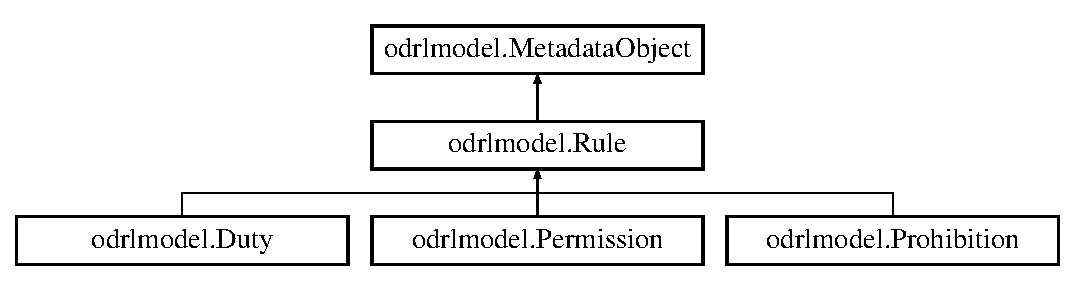
\includegraphics[height=3.000000cm]{classodrlmodel_1_1_rule}
\end{center}
\end{figure}
\subsection*{Public Member Functions}
\begin{DoxyCompactItemize}
\item 
\hyperlink{classodrlmodel_1_1_rule_acb4f2244902af08d9785f9456bb8820c}{Rule} ()
\item 
\hyperlink{classodrlmodel_1_1_rule_aaf7c5892139068d9561a50d4089b5bf6}{Rule} (String \-\_\-uri)
\item 
int \hyperlink{classodrlmodel_1_1_rule_a0d71548858ab50049760f914f61a0fc0}{get\-Kind\-Of\-Rule} ()
\item 
void \hyperlink{classodrlmodel_1_1_rule_ab1ff6bd55269f76b974eadfd92b668f8}{set\-Kind\-Of\-Rule} (int \-\_\-ikind)
\item 
List$<$ \hyperlink{classodrlmodel_1_1_action}{Action} $>$ \hyperlink{classodrlmodel_1_1_rule_aa781f875b164590aa2d8bb0bb8d88f94}{get\-Actions} ()
\item 
void \hyperlink{classodrlmodel_1_1_rule_a00027541128650f1f340f29934cebc65}{set\-Actions} (List$<$ \hyperlink{classodrlmodel_1_1_action}{Action} $>$ \-\_\-actions)
\item 
List$<$ \hyperlink{classodrlmodel_1_1_constraint}{Constraint} $>$ \hyperlink{classodrlmodel_1_1_rule_a65f3d362ba59a0c199d19586f3a1e871}{get\-Constraints} ()
\item 
void \hyperlink{classodrlmodel_1_1_rule_a28674bb5d2b9d33e855d3cecabe40fc4}{set\-Constraints} (List$<$ \hyperlink{classodrlmodel_1_1_constraint}{Constraint} $>$ \-\_\-constraints)
\item 
\hypertarget{classodrlmodel_1_1_rule_a30a8615e0a5fdbd4e2e9a43c006cdfa3}{void {\bfseries add\-Action} (\hyperlink{classodrlmodel_1_1_action}{Action} a)}\label{classodrlmodel_1_1_rule_a30a8615e0a5fdbd4e2e9a43c006cdfa3}

\item 
\hypertarget{classodrlmodel_1_1_rule_a9e7455aa5b0217bce0aec60c18986d04}{void {\bfseries add\-Constraint} (\hyperlink{classodrlmodel_1_1_constraint}{Constraint} a)}\label{classodrlmodel_1_1_rule_a9e7455aa5b0217bce0aec60c18986d04}

\item 
void \hyperlink{classodrlmodel_1_1_rule_ac165e23252d5bda726610ab28edede8b}{set\-Assignee} (\hyperlink{classodrlmodel_1_1_party}{Party} \-\_\-assignee)
\item 
\hyperlink{classodrlmodel_1_1_party}{Party} \hyperlink{classodrlmodel_1_1_rule_a10e7f232c1407bef1c5ed455b1261a8f}{get\-Assignee} ()
\item 
void \hyperlink{classodrlmodel_1_1_rule_a3b076086d56ef41f44198d18be14b70a}{set\-Assigner} (\hyperlink{classodrlmodel_1_1_party}{Party} \-\_\-assigner)
\item 
\hyperlink{classodrlmodel_1_1_party}{Party} \hyperlink{classodrlmodel_1_1_rule_a9e227b6b054757b2a88c83c41d619670}{get\-Assigner} ()
\item 
\hypertarget{classodrlmodel_1_1_rule_a4e33d42f26698a5ef54f0c6c652a4ded}{String {\bfseries to\-String} ()}\label{classodrlmodel_1_1_rule_a4e33d42f26698a5ef54f0c6c652a4ded}

\item 
\hypertarget{classodrlmodel_1_1_rule_a4a1f1badbc19cab2f3fb03af9868539b}{void {\bfseries set\-Target} (String target1)}\label{classodrlmodel_1_1_rule_a4a1f1badbc19cab2f3fb03af9868539b}

\end{DoxyCompactItemize}
\subsection*{Public Attributes}
\begin{DoxyCompactItemize}
\item 
\hypertarget{classodrlmodel_1_1_rule_a85913597237b11690fef60de3e33137e}{List$<$ \hyperlink{classodrlmodel_1_1_action}{Action} $>$ {\bfseries actions} = new Array\-List()}\label{classodrlmodel_1_1_rule_a85913597237b11690fef60de3e33137e}

\item 
\hypertarget{classodrlmodel_1_1_rule_a1ca369a8e3a30722213bd38d3e943e71}{List$<$ \hyperlink{classodrlmodel_1_1_constraint}{Constraint} $>$ {\bfseries constraints} = new Array\-List()}\label{classodrlmodel_1_1_rule_a1ca369a8e3a30722213bd38d3e943e71}

\item 
\hypertarget{classodrlmodel_1_1_rule_a016cea87c7c33f40b2f7af162fb96d71}{String {\bfseries target} =\char`\"{}\char`\"{}}\label{classodrlmodel_1_1_rule_a016cea87c7c33f40b2f7af162fb96d71}

\end{DoxyCompactItemize}
\subsection*{Static Public Attributes}
\begin{DoxyCompactItemize}
\item 
\hypertarget{classodrlmodel_1_1_rule_a60761e0d1bbaf52812face396feb6985}{static final int {\bfseries R\-U\-L\-E\-\_\-\-P\-E\-R\-M\-I\-S\-S\-I\-O\-N} = 0}\label{classodrlmodel_1_1_rule_a60761e0d1bbaf52812face396feb6985}

\item 
\hypertarget{classodrlmodel_1_1_rule_abd05faac196bb56c1edf254268a2df8e}{static final int {\bfseries R\-U\-L\-E\-\_\-\-P\-R\-O\-H\-I\-B\-I\-T\-I\-O\-N} = 1}\label{classodrlmodel_1_1_rule_abd05faac196bb56c1edf254268a2df8e}

\item 
\hypertarget{classodrlmodel_1_1_rule_acc7b2c95eee78645cd4614c8202c96ec}{static final int {\bfseries R\-U\-L\-E\-\_\-\-D\-U\-T\-Y} = 2}\label{classodrlmodel_1_1_rule_acc7b2c95eee78645cd4614c8202c96ec}

\end{DoxyCompactItemize}
\subsection*{Protected Member Functions}
\begin{DoxyCompactItemize}
\item 
String \hyperlink{classodrlmodel_1_1_rule_ab794be33eac213d7ebc7124baaf479c3}{get\-Kind\-Of\-Rule\-String} ()
\end{DoxyCompactItemize}
\subsection*{Protected Attributes}
\begin{DoxyCompactItemize}
\item 
\hypertarget{classodrlmodel_1_1_rule_a22aba6ee5f6981c1c487cf5d638c8941}{\hyperlink{classodrlmodel_1_1_party}{Party} {\bfseries assignee} =null}\label{classodrlmodel_1_1_rule_a22aba6ee5f6981c1c487cf5d638c8941}

\item 
\hypertarget{classodrlmodel_1_1_rule_a5494d7ff153d6047be45c9950ac8877b}{\hyperlink{classodrlmodel_1_1_party}{Party} {\bfseries assigner} = null}\label{classodrlmodel_1_1_rule_a5494d7ff153d6047be45c9950ac8877b}

\end{DoxyCompactItemize}


\subsection{Detailed Description}
This class represents a simple O\-D\-R\-L rule \hyperlink{classodrlmodel_1_1_rule}{Rule} is an abstract common ancestor to Permissions, Prohibitions and Duties. A \hyperlink{classodrlmodel_1_1_rule}{Rule} (reduced version of the O\-D\-R\-L \hyperlink{classodrlmodel_1_1_rule}{Rule}) is made of\-:
\begin{DoxyItemize}
\item Zero or more actions
\item Zero or more constraints
\item Zero or one assignee (party enjoying the permission/prohibition/duty)
\item Zero or one target (object over which the rule applies)
\item Zero or one assigner (party assigning the rule) \begin{DoxyAuthor}{Author}
Victor Rodriguez Doncel at O\-E\-G-\/\-U\-P\-M 2014 
\end{DoxyAuthor}

\end{DoxyItemize}

\subsection{Constructor \& Destructor Documentation}
\hypertarget{classodrlmodel_1_1_rule_acb4f2244902af08d9785f9456bb8820c}{\index{odrlmodel\-::\-Rule@{odrlmodel\-::\-Rule}!Rule@{Rule}}
\index{Rule@{Rule}!odrlmodel::Rule@{odrlmodel\-::\-Rule}}
\subsubsection[{Rule}]{\setlength{\rightskip}{0pt plus 5cm}odrlmodel.\-Rule.\-Rule (
\begin{DoxyParamCaption}
{}
\end{DoxyParamCaption}
)}}\label{classodrlmodel_1_1_rule_acb4f2244902af08d9785f9456bb8820c}
\hyperlink{classodrlmodel_1_1_rule}{Rule} constructor with a random U\-R\-I in the default namespace A rule is by default a constructor \hypertarget{classodrlmodel_1_1_rule_aaf7c5892139068d9561a50d4089b5bf6}{\index{odrlmodel\-::\-Rule@{odrlmodel\-::\-Rule}!Rule@{Rule}}
\index{Rule@{Rule}!odrlmodel::Rule@{odrlmodel\-::\-Rule}}
\subsubsection[{Rule}]{\setlength{\rightskip}{0pt plus 5cm}odrlmodel.\-Rule.\-Rule (
\begin{DoxyParamCaption}
\item[{String}]{\-\_\-uri}
\end{DoxyParamCaption}
)}}\label{classodrlmodel_1_1_rule_aaf7c5892139068d9561a50d4089b5bf6}
\hyperlink{classodrlmodel_1_1_rule}{Rule} constructor with a given U\-R\-I 
\begin{DoxyParams}{Parameters}
{\em \-\_\-uri} & A valid U\-R\-I. Can be an empty string (anonymous source) \\
\hline
\end{DoxyParams}


\subsection{Member Function Documentation}
\hypertarget{classodrlmodel_1_1_rule_aa781f875b164590aa2d8bb0bb8d88f94}{\index{odrlmodel\-::\-Rule@{odrlmodel\-::\-Rule}!get\-Actions@{get\-Actions}}
\index{get\-Actions@{get\-Actions}!odrlmodel::Rule@{odrlmodel\-::\-Rule}}
\subsubsection[{get\-Actions}]{\setlength{\rightskip}{0pt plus 5cm}List$<${\bf Action}$>$ odrlmodel.\-Rule.\-get\-Actions (
\begin{DoxyParamCaption}
{}
\end{DoxyParamCaption}
)}}\label{classodrlmodel_1_1_rule_aa781f875b164590aa2d8bb0bb8d88f94}
Gets the actions associated to this rule \hypertarget{classodrlmodel_1_1_rule_a10e7f232c1407bef1c5ed455b1261a8f}{\index{odrlmodel\-::\-Rule@{odrlmodel\-::\-Rule}!get\-Assignee@{get\-Assignee}}
\index{get\-Assignee@{get\-Assignee}!odrlmodel::Rule@{odrlmodel\-::\-Rule}}
\subsubsection[{get\-Assignee}]{\setlength{\rightskip}{0pt plus 5cm}{\bf Party} odrlmodel.\-Rule.\-get\-Assignee (
\begin{DoxyParamCaption}
{}
\end{DoxyParamCaption}
)}}\label{classodrlmodel_1_1_rule_a10e7f232c1407bef1c5ed455b1261a8f}
Gets the assignee of the rule. \begin{DoxyReturn}{Returns}
The assignee 
\end{DoxyReturn}
\hypertarget{classodrlmodel_1_1_rule_a9e227b6b054757b2a88c83c41d619670}{\index{odrlmodel\-::\-Rule@{odrlmodel\-::\-Rule}!get\-Assigner@{get\-Assigner}}
\index{get\-Assigner@{get\-Assigner}!odrlmodel::Rule@{odrlmodel\-::\-Rule}}
\subsubsection[{get\-Assigner}]{\setlength{\rightskip}{0pt plus 5cm}{\bf Party} odrlmodel.\-Rule.\-get\-Assigner (
\begin{DoxyParamCaption}
{}
\end{DoxyParamCaption}
)}}\label{classodrlmodel_1_1_rule_a9e227b6b054757b2a88c83c41d619670}
Gets the assigner of the rule. \begin{DoxyReturn}{Returns}
The assigner 
\end{DoxyReturn}
\hypertarget{classodrlmodel_1_1_rule_a65f3d362ba59a0c199d19586f3a1e871}{\index{odrlmodel\-::\-Rule@{odrlmodel\-::\-Rule}!get\-Constraints@{get\-Constraints}}
\index{get\-Constraints@{get\-Constraints}!odrlmodel::Rule@{odrlmodel\-::\-Rule}}
\subsubsection[{get\-Constraints}]{\setlength{\rightskip}{0pt plus 5cm}List$<${\bf Constraint}$>$ odrlmodel.\-Rule.\-get\-Constraints (
\begin{DoxyParamCaption}
{}
\end{DoxyParamCaption}
)}}\label{classodrlmodel_1_1_rule_a65f3d362ba59a0c199d19586f3a1e871}
Gets the list of constraints the rule has. \begin{DoxyReturn}{Returns}
List of constraints 
\end{DoxyReturn}
\hypertarget{classodrlmodel_1_1_rule_a0d71548858ab50049760f914f61a0fc0}{\index{odrlmodel\-::\-Rule@{odrlmodel\-::\-Rule}!get\-Kind\-Of\-Rule@{get\-Kind\-Of\-Rule}}
\index{get\-Kind\-Of\-Rule@{get\-Kind\-Of\-Rule}!odrlmodel::Rule@{odrlmodel\-::\-Rule}}
\subsubsection[{get\-Kind\-Of\-Rule}]{\setlength{\rightskip}{0pt plus 5cm}int odrlmodel.\-Rule.\-get\-Kind\-Of\-Rule (
\begin{DoxyParamCaption}
{}
\end{DoxyParamCaption}
)}}\label{classodrlmodel_1_1_rule_a0d71548858ab50049760f914f61a0fc0}
Gets the kind of the rule \begin{DoxyReturn}{Returns}
either Rule.\-R\-U\-L\-E\-\_\-\-P\-E\-R\-M\-I\-S\-S\-I\-O\-N, Rule.\-R\-U\-L\-E\-\_\-\-P\-R\-O\-H\-I\-B\-I\-T\-I\-O\-N or Rule.\-R\-U\-L\-E\-\_\-\-D\-U\-T\-Y 
\end{DoxyReturn}
\hypertarget{classodrlmodel_1_1_rule_ab794be33eac213d7ebc7124baaf479c3}{\index{odrlmodel\-::\-Rule@{odrlmodel\-::\-Rule}!get\-Kind\-Of\-Rule\-String@{get\-Kind\-Of\-Rule\-String}}
\index{get\-Kind\-Of\-Rule\-String@{get\-Kind\-Of\-Rule\-String}!odrlmodel::Rule@{odrlmodel\-::\-Rule}}
\subsubsection[{get\-Kind\-Of\-Rule\-String}]{\setlength{\rightskip}{0pt plus 5cm}String odrlmodel.\-Rule.\-get\-Kind\-Of\-Rule\-String (
\begin{DoxyParamCaption}
{}
\end{DoxyParamCaption}
)\hspace{0.3cm}{\ttfamily [protected]}}}\label{classodrlmodel_1_1_rule_ab794be33eac213d7ebc7124baaf479c3}
Gets an string describing the kind of the rule \begin{DoxyReturn}{Returns}
either \char`\"{}\-Permission\char`\"{}, or \char`\"{}\-Prohibition\char`\"{} or \char`\"{}\-Duty\char`\"{} -\/empty if unkown kind. 
\end{DoxyReturn}
\hypertarget{classodrlmodel_1_1_rule_a00027541128650f1f340f29934cebc65}{\index{odrlmodel\-::\-Rule@{odrlmodel\-::\-Rule}!set\-Actions@{set\-Actions}}
\index{set\-Actions@{set\-Actions}!odrlmodel::Rule@{odrlmodel\-::\-Rule}}
\subsubsection[{set\-Actions}]{\setlength{\rightskip}{0pt plus 5cm}void odrlmodel.\-Rule.\-set\-Actions (
\begin{DoxyParamCaption}
\item[{List$<$ {\bf Action} $>$}]{\-\_\-actions}
\end{DoxyParamCaption}
)}}\label{classodrlmodel_1_1_rule_a00027541128650f1f340f29934cebc65}
Sets the actions referred by this rule 
\begin{DoxyParams}{Parameters}
{\em \-\_\-actions} & List of actions \\
\hline
\end{DoxyParams}
\hypertarget{classodrlmodel_1_1_rule_ac165e23252d5bda726610ab28edede8b}{\index{odrlmodel\-::\-Rule@{odrlmodel\-::\-Rule}!set\-Assignee@{set\-Assignee}}
\index{set\-Assignee@{set\-Assignee}!odrlmodel::Rule@{odrlmodel\-::\-Rule}}
\subsubsection[{set\-Assignee}]{\setlength{\rightskip}{0pt plus 5cm}void odrlmodel.\-Rule.\-set\-Assignee (
\begin{DoxyParamCaption}
\item[{{\bf Party}}]{\-\_\-assignee}
\end{DoxyParamCaption}
)}}\label{classodrlmodel_1_1_rule_ac165e23252d5bda726610ab28edede8b}
Sets the assignee of the rule 
\begin{DoxyParams}{Parameters}
{\em \-\_\-assignee} & \\
\hline
\end{DoxyParams}
\hypertarget{classodrlmodel_1_1_rule_a3b076086d56ef41f44198d18be14b70a}{\index{odrlmodel\-::\-Rule@{odrlmodel\-::\-Rule}!set\-Assigner@{set\-Assigner}}
\index{set\-Assigner@{set\-Assigner}!odrlmodel::Rule@{odrlmodel\-::\-Rule}}
\subsubsection[{set\-Assigner}]{\setlength{\rightskip}{0pt plus 5cm}void odrlmodel.\-Rule.\-set\-Assigner (
\begin{DoxyParamCaption}
\item[{{\bf Party}}]{\-\_\-assigner}
\end{DoxyParamCaption}
)}}\label{classodrlmodel_1_1_rule_a3b076086d56ef41f44198d18be14b70a}
Sets the assigner of the rule 
\begin{DoxyParams}{Parameters}
{\em \-\_\-assigner} & \\
\hline
\end{DoxyParams}
\hypertarget{classodrlmodel_1_1_rule_a28674bb5d2b9d33e855d3cecabe40fc4}{\index{odrlmodel\-::\-Rule@{odrlmodel\-::\-Rule}!set\-Constraints@{set\-Constraints}}
\index{set\-Constraints@{set\-Constraints}!odrlmodel::Rule@{odrlmodel\-::\-Rule}}
\subsubsection[{set\-Constraints}]{\setlength{\rightskip}{0pt plus 5cm}void odrlmodel.\-Rule.\-set\-Constraints (
\begin{DoxyParamCaption}
\item[{List$<$ {\bf Constraint} $>$}]{\-\_\-constraints}
\end{DoxyParamCaption}
)}}\label{classodrlmodel_1_1_rule_a28674bb5d2b9d33e855d3cecabe40fc4}
Sets the constraints for this rule to apply 
\begin{DoxyParams}{Parameters}
{\em \-\_\-constraints} & List of constratins \\
\hline
\end{DoxyParams}
\hypertarget{classodrlmodel_1_1_rule_ab1ff6bd55269f76b974eadfd92b668f8}{\index{odrlmodel\-::\-Rule@{odrlmodel\-::\-Rule}!set\-Kind\-Of\-Rule@{set\-Kind\-Of\-Rule}}
\index{set\-Kind\-Of\-Rule@{set\-Kind\-Of\-Rule}!odrlmodel::Rule@{odrlmodel\-::\-Rule}}
\subsubsection[{set\-Kind\-Of\-Rule}]{\setlength{\rightskip}{0pt plus 5cm}void odrlmodel.\-Rule.\-set\-Kind\-Of\-Rule (
\begin{DoxyParamCaption}
\item[{int}]{\-\_\-ikind}
\end{DoxyParamCaption}
)}}\label{classodrlmodel_1_1_rule_ab1ff6bd55269f76b974eadfd92b668f8}
Sets the kind of rule 
\begin{DoxyParams}{Parameters}
{\em \-\_\-ikind} & either Rule.\-R\-U\-L\-E\-\_\-\-P\-E\-R\-M\-I\-S\-S\-I\-O\-N, Rule.\-R\-U\-L\-E\-\_\-\-P\-R\-O\-H\-I\-B\-I\-T\-I\-O\-N or Rule.\-R\-U\-L\-E\-\_\-\-D\-U\-T\-Y \\
\hline
\end{DoxyParams}


The documentation for this class was generated from the following file\-:\begin{DoxyCompactItemize}
\item 
src/odrlmodel/Rule.\-java\end{DoxyCompactItemize}

\addcontentsline{toc}{part}{Index}
\printindex
\end{document}
